% CVM 2027 anonymous review manuscript, migrated 2026-10-25.
% Revision review draft; see the separate submission checklist before upload.
\documentclass[10pt,twocolumn,letterpaper]{article}
\usepackage[T1]{fontenc}
\usepackage{cvm}
\usepackage{times}
\usepackage{epsfig}
\usepackage{graphicx}
\usepackage{amsmath,amssymb,booktabs,multirow,url,cite,placeins,flushend}
\usepackage[pagebackref=true,breaklinks=true,letterpaper=true,colorlinks,bookmarks=false]{hyperref}
\hypersetup{pdftitle={Native-Unit Selection for Visual Token Compression},pdfauthor={},pdfsubject={},pdfkeywords={}}
\newcommand{\keywords}[1]{{\bf \emph{Keywords: #1}}}
% Keep the official placeholder until the submission portal assigns the real ID.
\def\cvmPaperID{****}
\def\httilde{\mbox{\tt\raisebox{-.5ex}{\symbol{126}}}}
\ifcvmfinal\pagestyle{empty}\fi
\begin{document}
\title{Native-Unit Selection for Visual Token Compression}
\author{}
\maketitle

\begin{abstract}
Visual token compression requires a budget and a representation for ranking candidate units. We study norm-based selection at native visual merger and projector inputs and outputs. Rank-Before-Merge (RBM) selects complete native units without training or changing learned projection weights. At 25\% retention, its deployed adapters exceed Post-L2 on all nine text-dense model--benchmark pairs across Qwen3-VL, Qwen2.5-VL, and InternVL3. Qwen3-VL controls favor main-output selection on DocVQA and GQA but final-input selection on TextVQA and OCRBench. Under shared attention on full splits, RBM trails FastV by 1.32 percentage points on TextVQA but exceeds it by 157 points out of 1,000 on OCRBench. RBM exceeds Hi-Lo Prune by 8.83 points on TextVQA; their OCRBench difference is $-2$ [$-31$, 27] points out of 1,000. Retention curves and a 500-question DocVQA stress test further probe the quality tradeoffs. On fixed samples of 100 questions per task, RBM at 50\% retention reaches 95\% of observed uncompressed quality with 25.4\% and 10.0\% lower median request latency on TextVQA and OCRBench. These results connect task-dependent selection quality with complete-request cost.
\end{abstract}

\keywords{Vision-language models, visual token compression, token selection, document understanding, efficient inference}

\section{Introduction}
High-resolution vision--language models convert many image patches into visual inputs for a language model. Native spatial mergers and projectors impose a model-specific unit structure, so additional compression must choose both how many units to retain and which representation to use for selection. Feature magnitudes can change across these operators, giving different retained sets at the same final token budget. We ask how this choice affects text-dense and object-centered visual question answering.

Rank-Before-Merge (RBM) ranks complete native units using feature norms at the inputs of native mergers or projectors. It reuses their learned weights and output dimensions and introduces no training. The implementation uses a shared unit mask across Qwen3-VL's main and auxiliary streams and model-specific adapters for Qwen2.5-VL and InternVL3.

We evaluate three model families on full TextVQA, DocVQA, OCRBench, and GQA splits at 25\% retention. We then decompose the Qwen3-VL design into an early-input selector, a final-input selector, and two output selectors that score either the main stream alone or its concatenation with auxiliary streams. Additional Qwen3-VL experiments compare RBM with FastV and Hi-Lo Prune, sweep 25/50/75\% retention, stress document understanding at a shared resolution cap, and measure complete requests. This design connects representation choices with accuracy and actual execution cost.

\begin{figure*}[t]
\centering
% Layout-only crops of the original author-supplied PNG; no pixel edits.
% Native image dimensions: 1908 x 824 pixels at the default 72 dpi.
% Omit the independent bottom slogan and the upper-right causal label.
\resizebox{\textwidth}{!}{%
\setlength{\unitlength}{1bp}%
\begin{picture}(1908,750)
\put(0,601){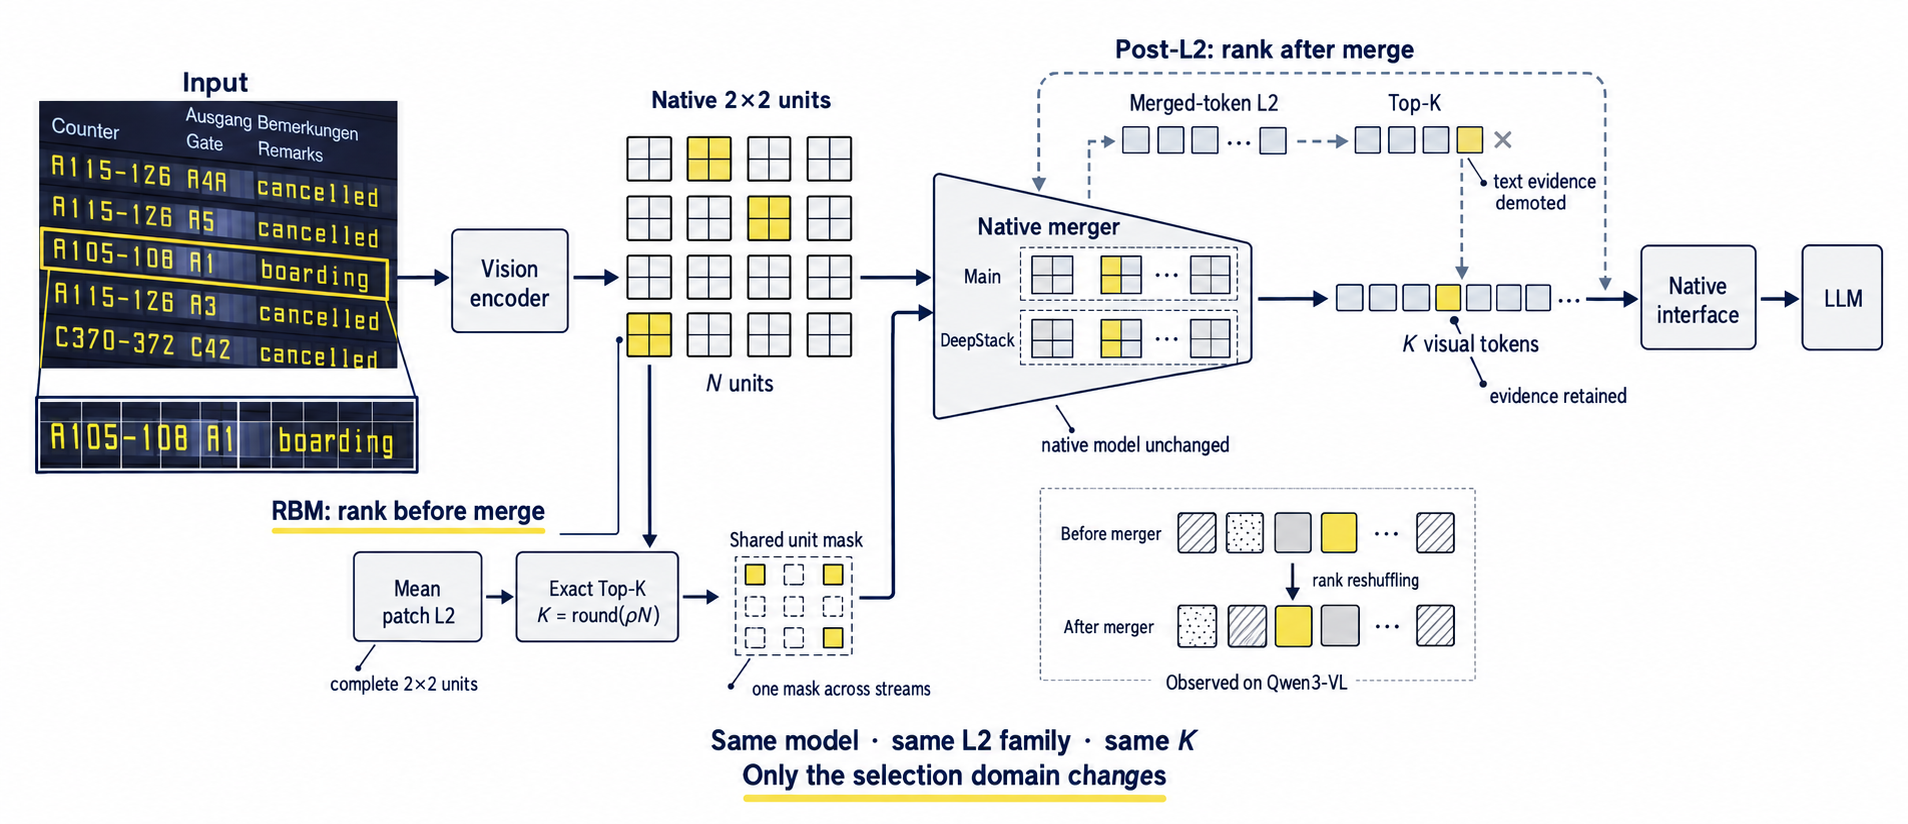
\includegraphics[viewport=0 675 1908 824,clip]{figs/fig1_user_20260915_v2.png}}
\put(0,529){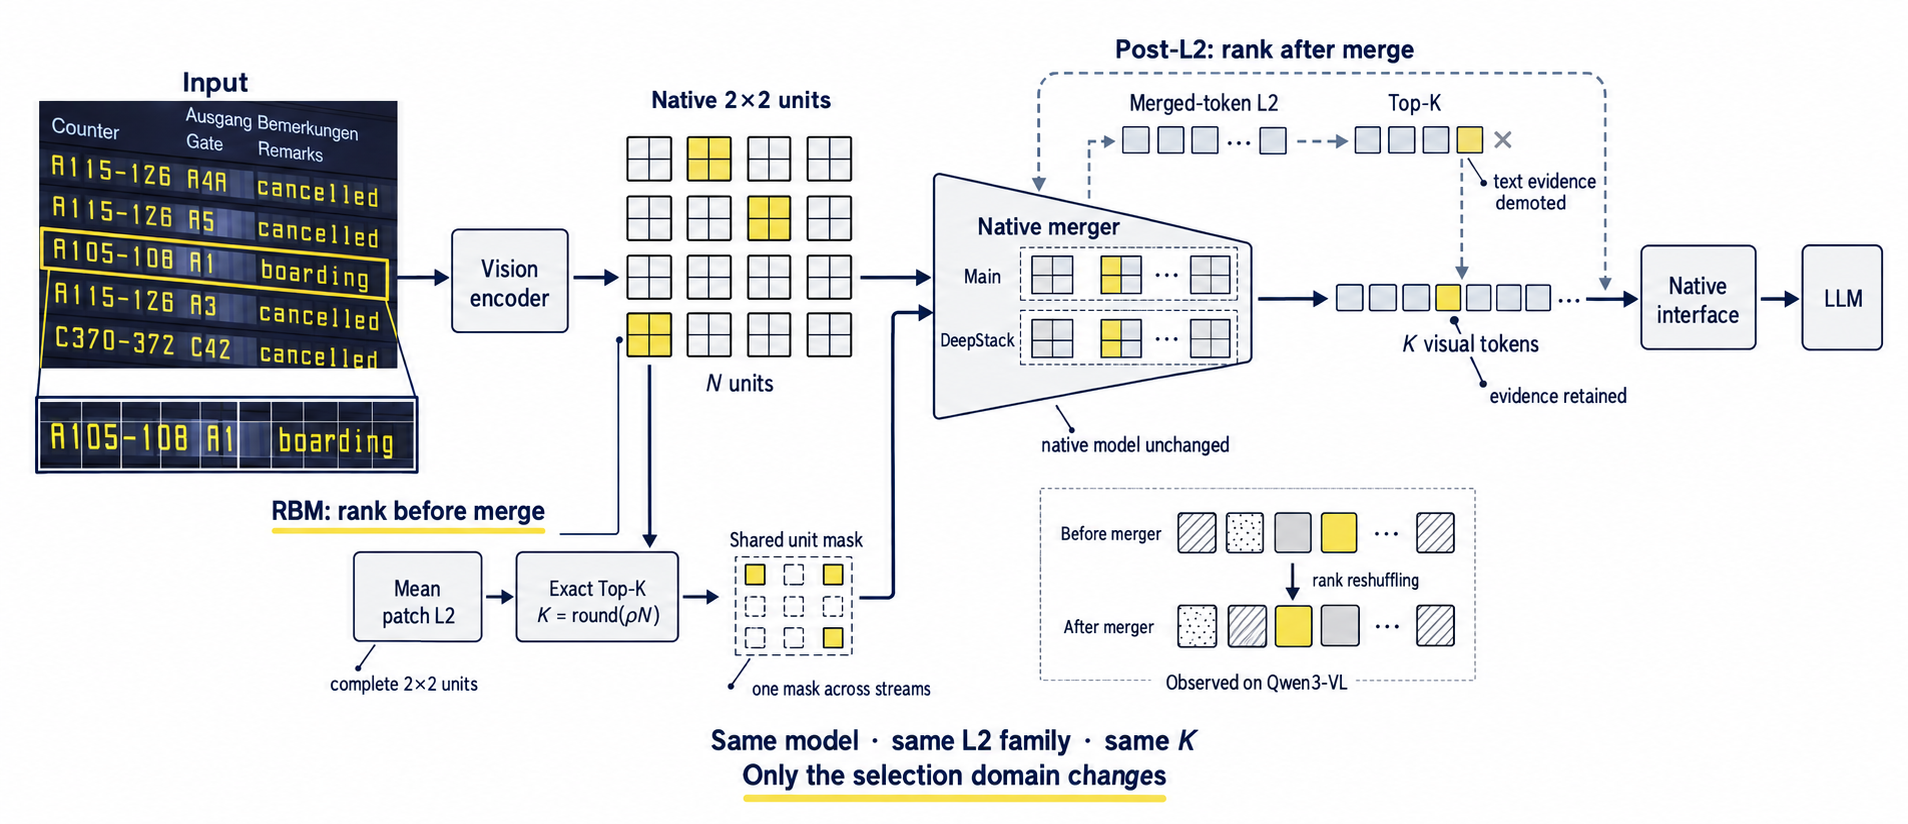
\includegraphics[viewport=0 603 1470 675,clip]{figs/fig1_user_20260915_v2.png}}
\put(1606,529){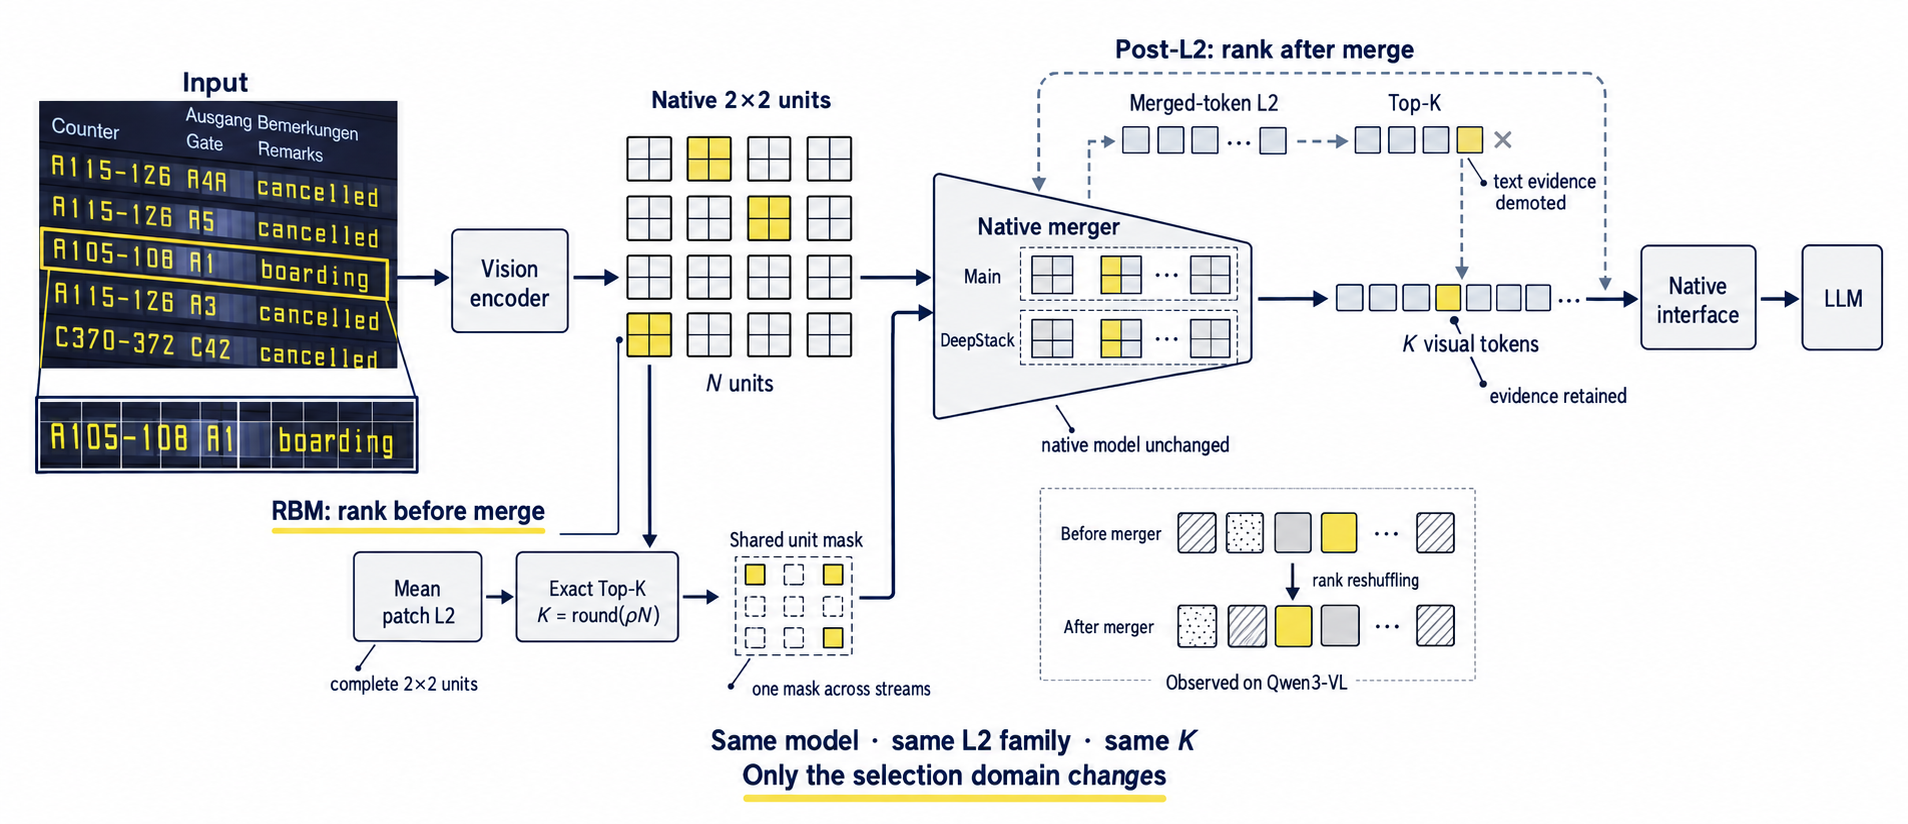
\includegraphics[viewport=1606 603 1908 675,clip]{figs/fig1_user_20260915_v2.png}}
\put(0,325){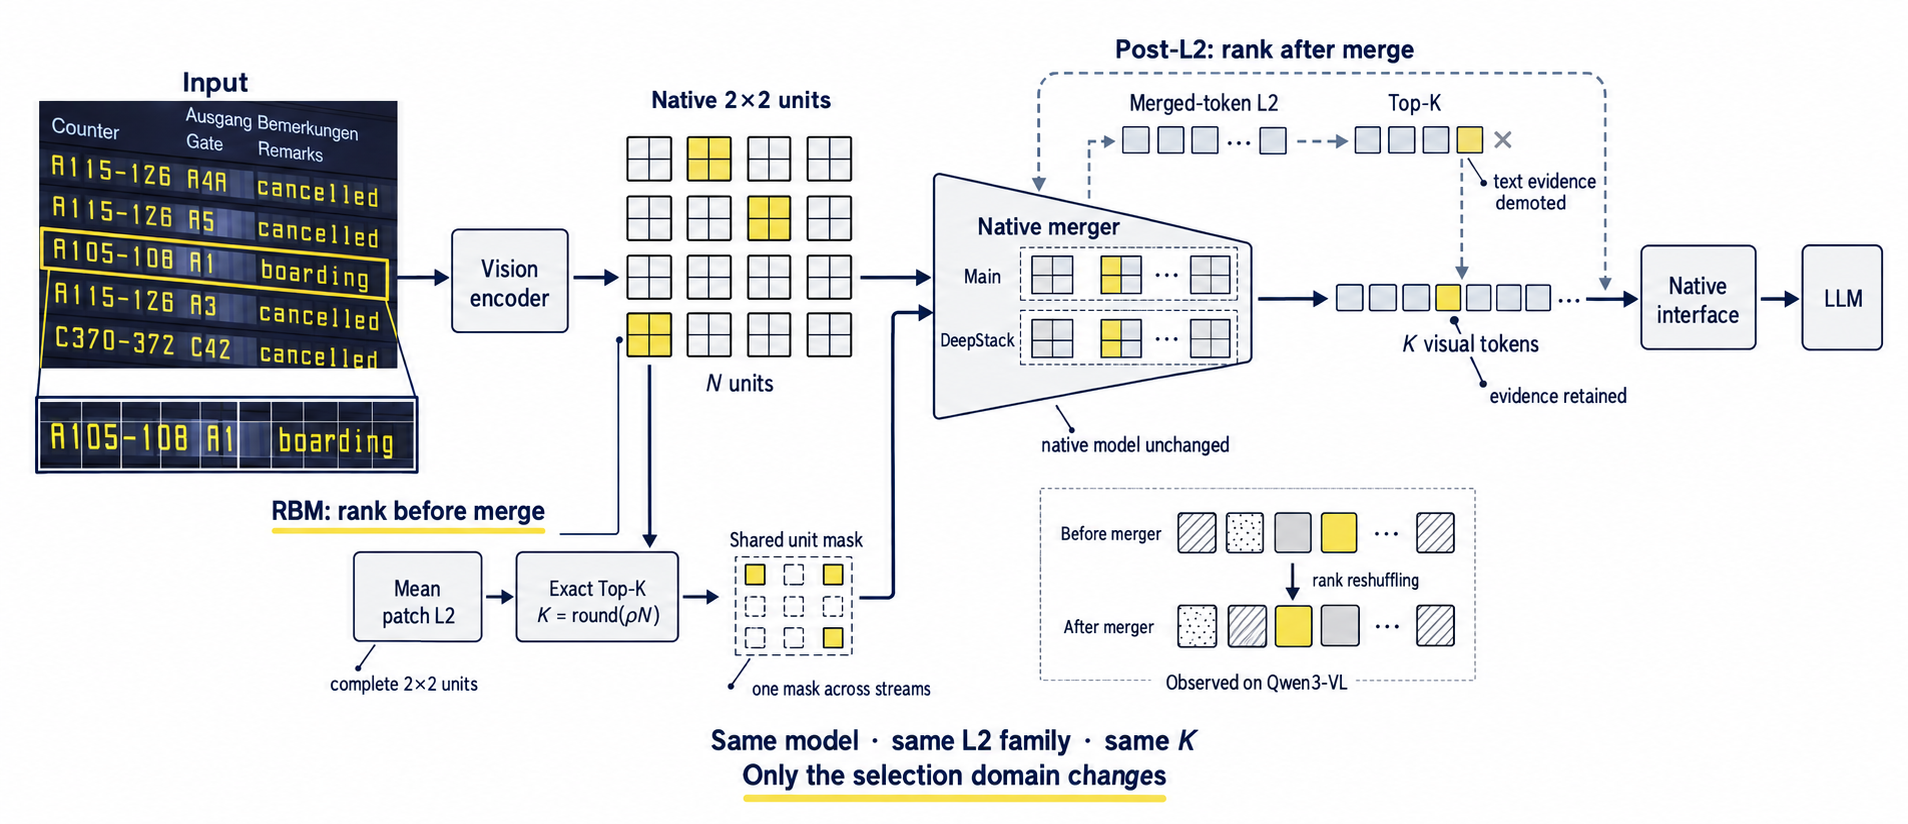
\includegraphics[viewport=0 399 1908 603,clip]{figs/fig1_user_20260915_v2.png}}
\put(0,275){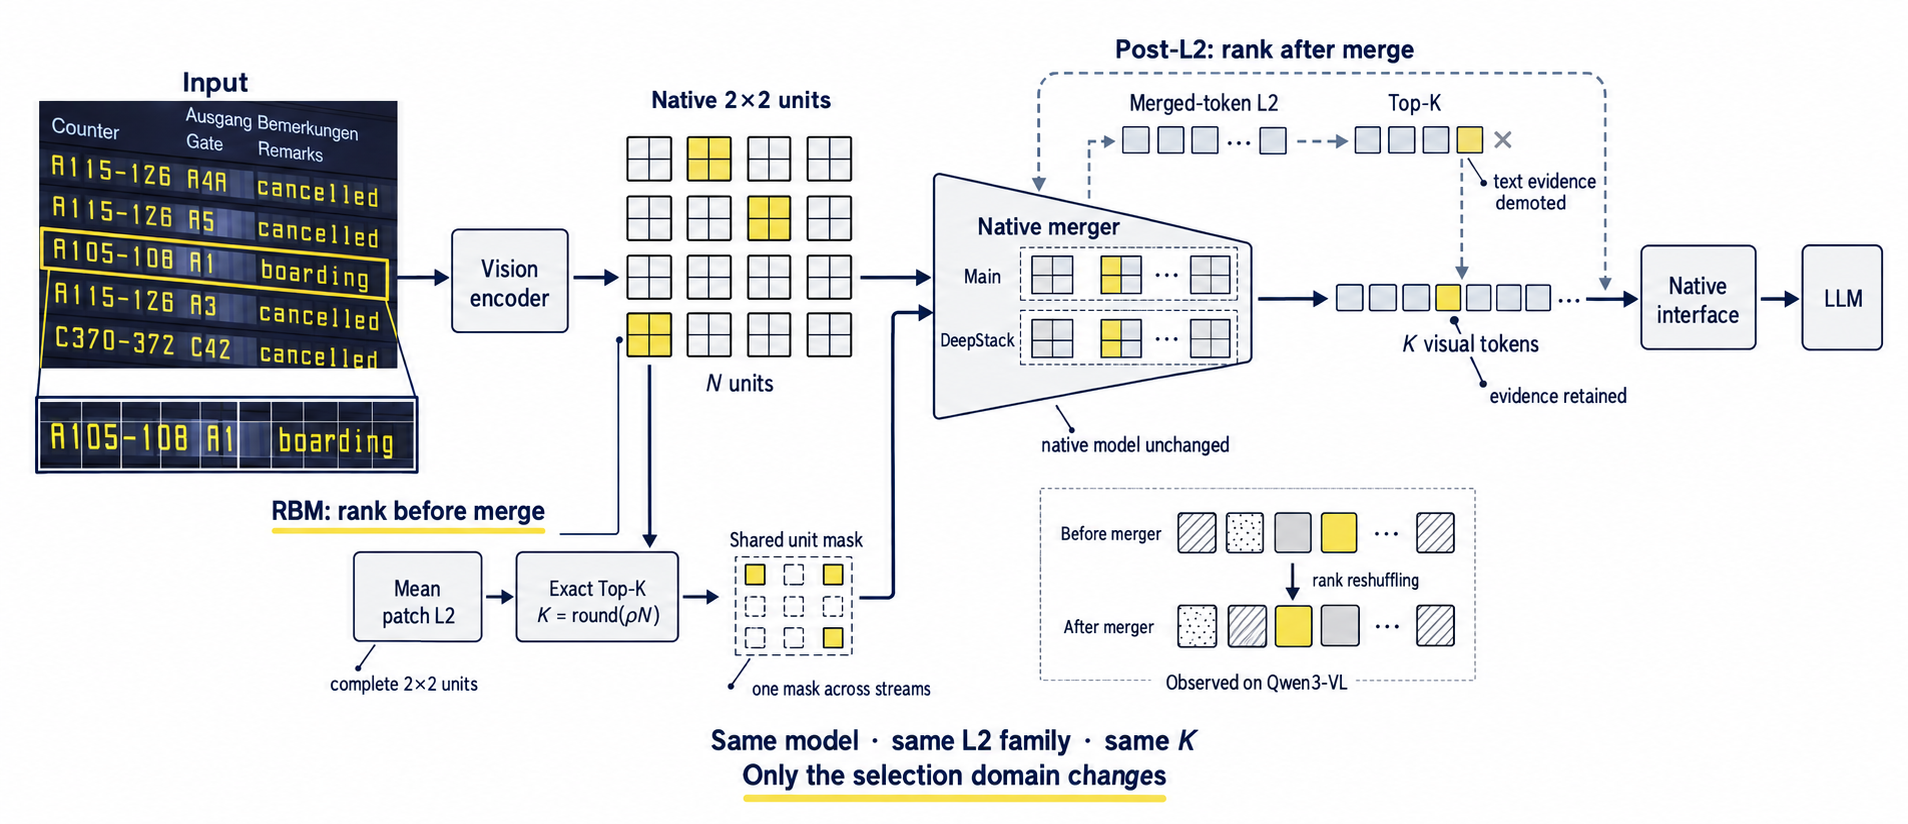
\includegraphics[viewport=0 349 1000 399,clip]{figs/fig1_user_20260915_v2.png}}
\put(1270,275){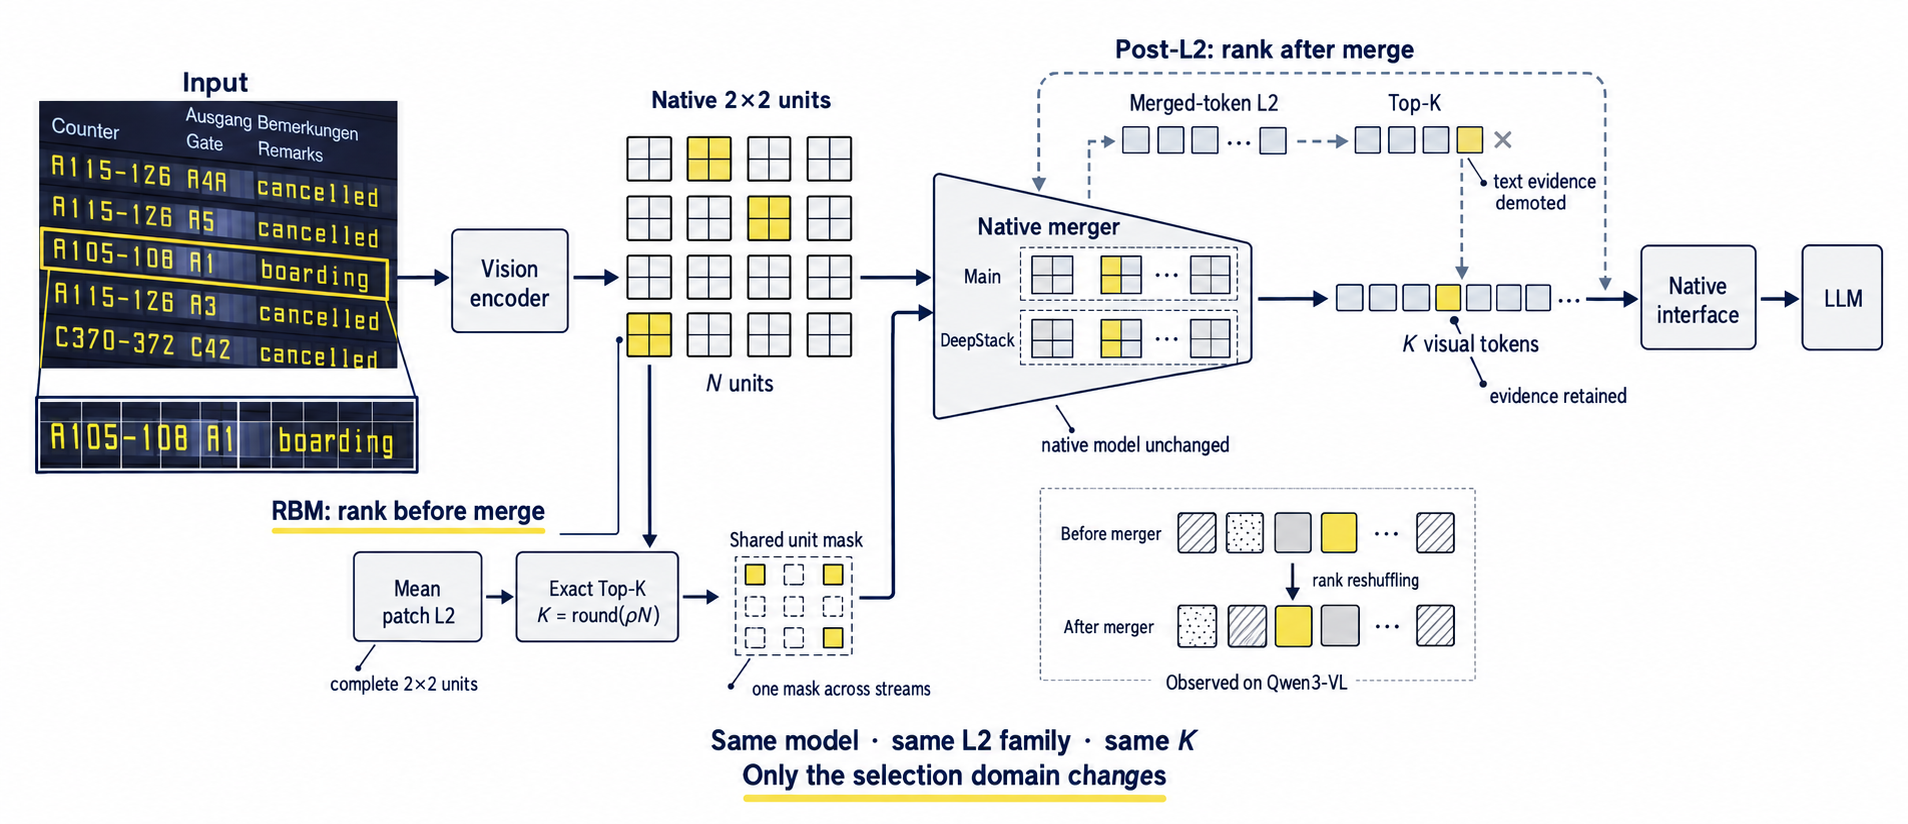
\includegraphics[viewport=1270 349 1908 399,clip]{figs/fig1_user_20260915_v2.png}}
\put(0,35){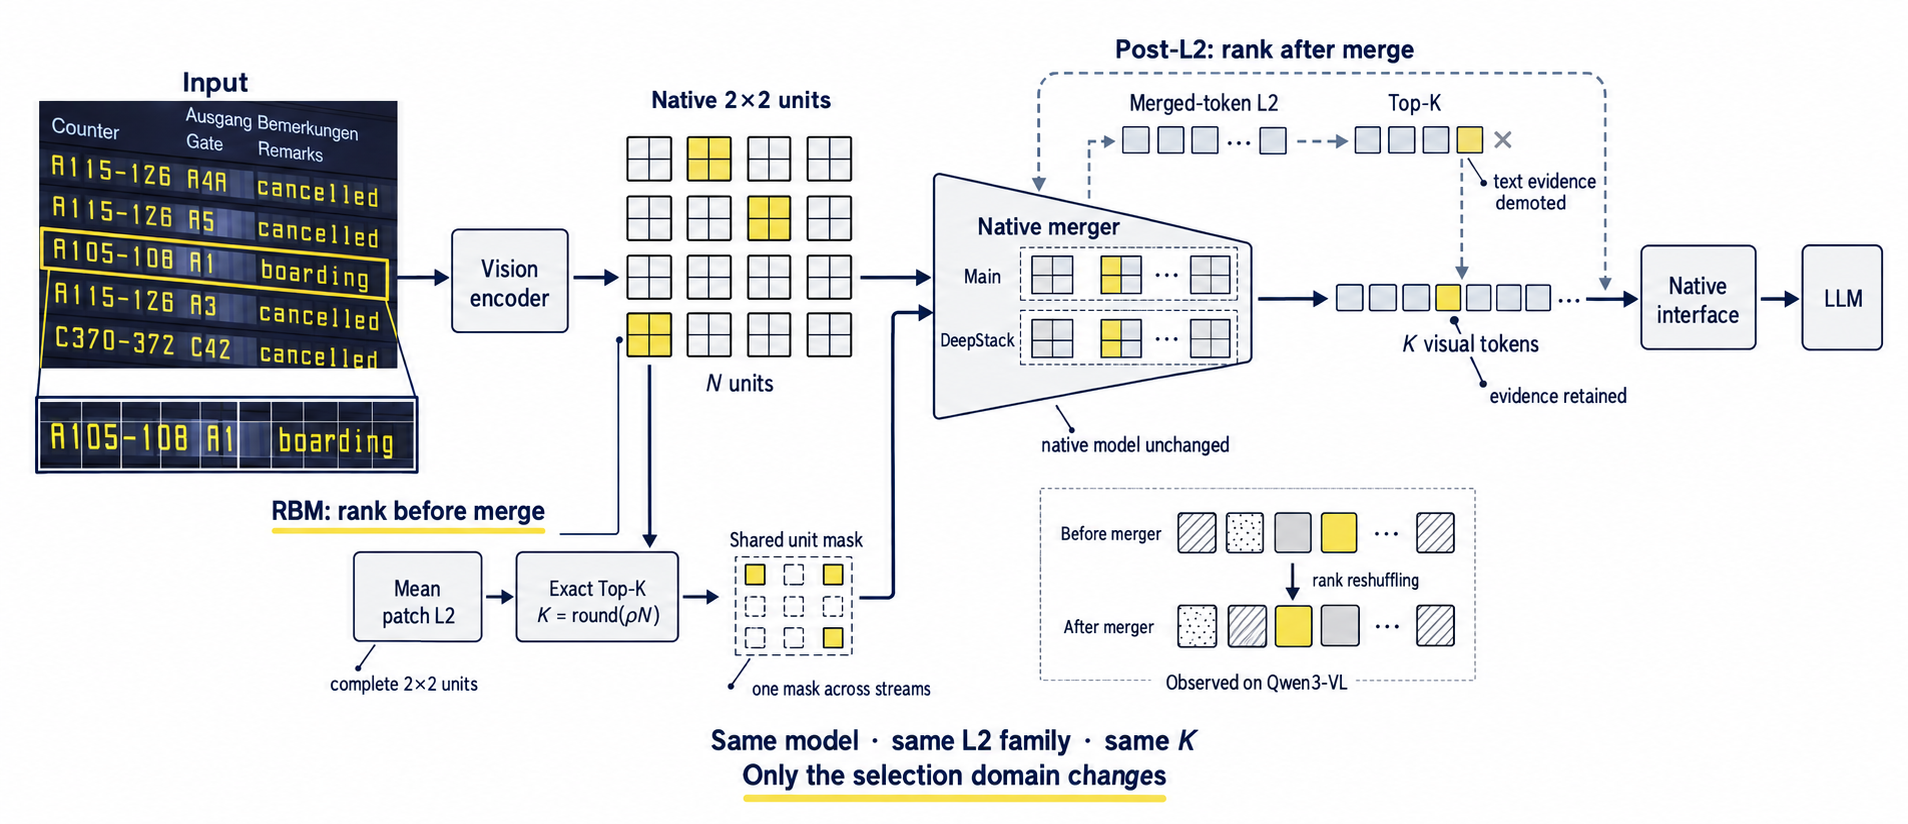
\includegraphics[viewport=0 109 1908 349,clip]{figs/fig1_user_20260915_v2.png}}
\put(1472,556){\makebox(132,0)[l]{\fontsize{23}{25}\selectfont Post-merger}}
\put(1472,531){\makebox(132,0)[l]{\fontsize{23}{25}\selectfont selected units}}
\put(1035,307){\makebox(225,0)[l]{\fontsize{23}{25}\selectfont Native merger}}
\put(1035,282){\makebox(225,0)[l]{\fontsize{23}{25}\selectfont weights reused}}
\put(954,7){\makebox(0,0){\fontsize{30}{34}\selectfont Selection uses different feature representations}}
\end{picture}%
}

\caption{\label{fig:overview}Native-unit ranking at merger inputs. RBM selects complete units and reuses the native merger weights; the same retained identities align the surviving output streams. Qwen3-VL uses the layer-8 deepstack input for deployed RBM and the final-block main-merger input for the Pre-final variant. The HuggingFace implementation gathers retained outputs after full visual computation.}
\end{figure*}

\begin{figure*}[t]
\centering
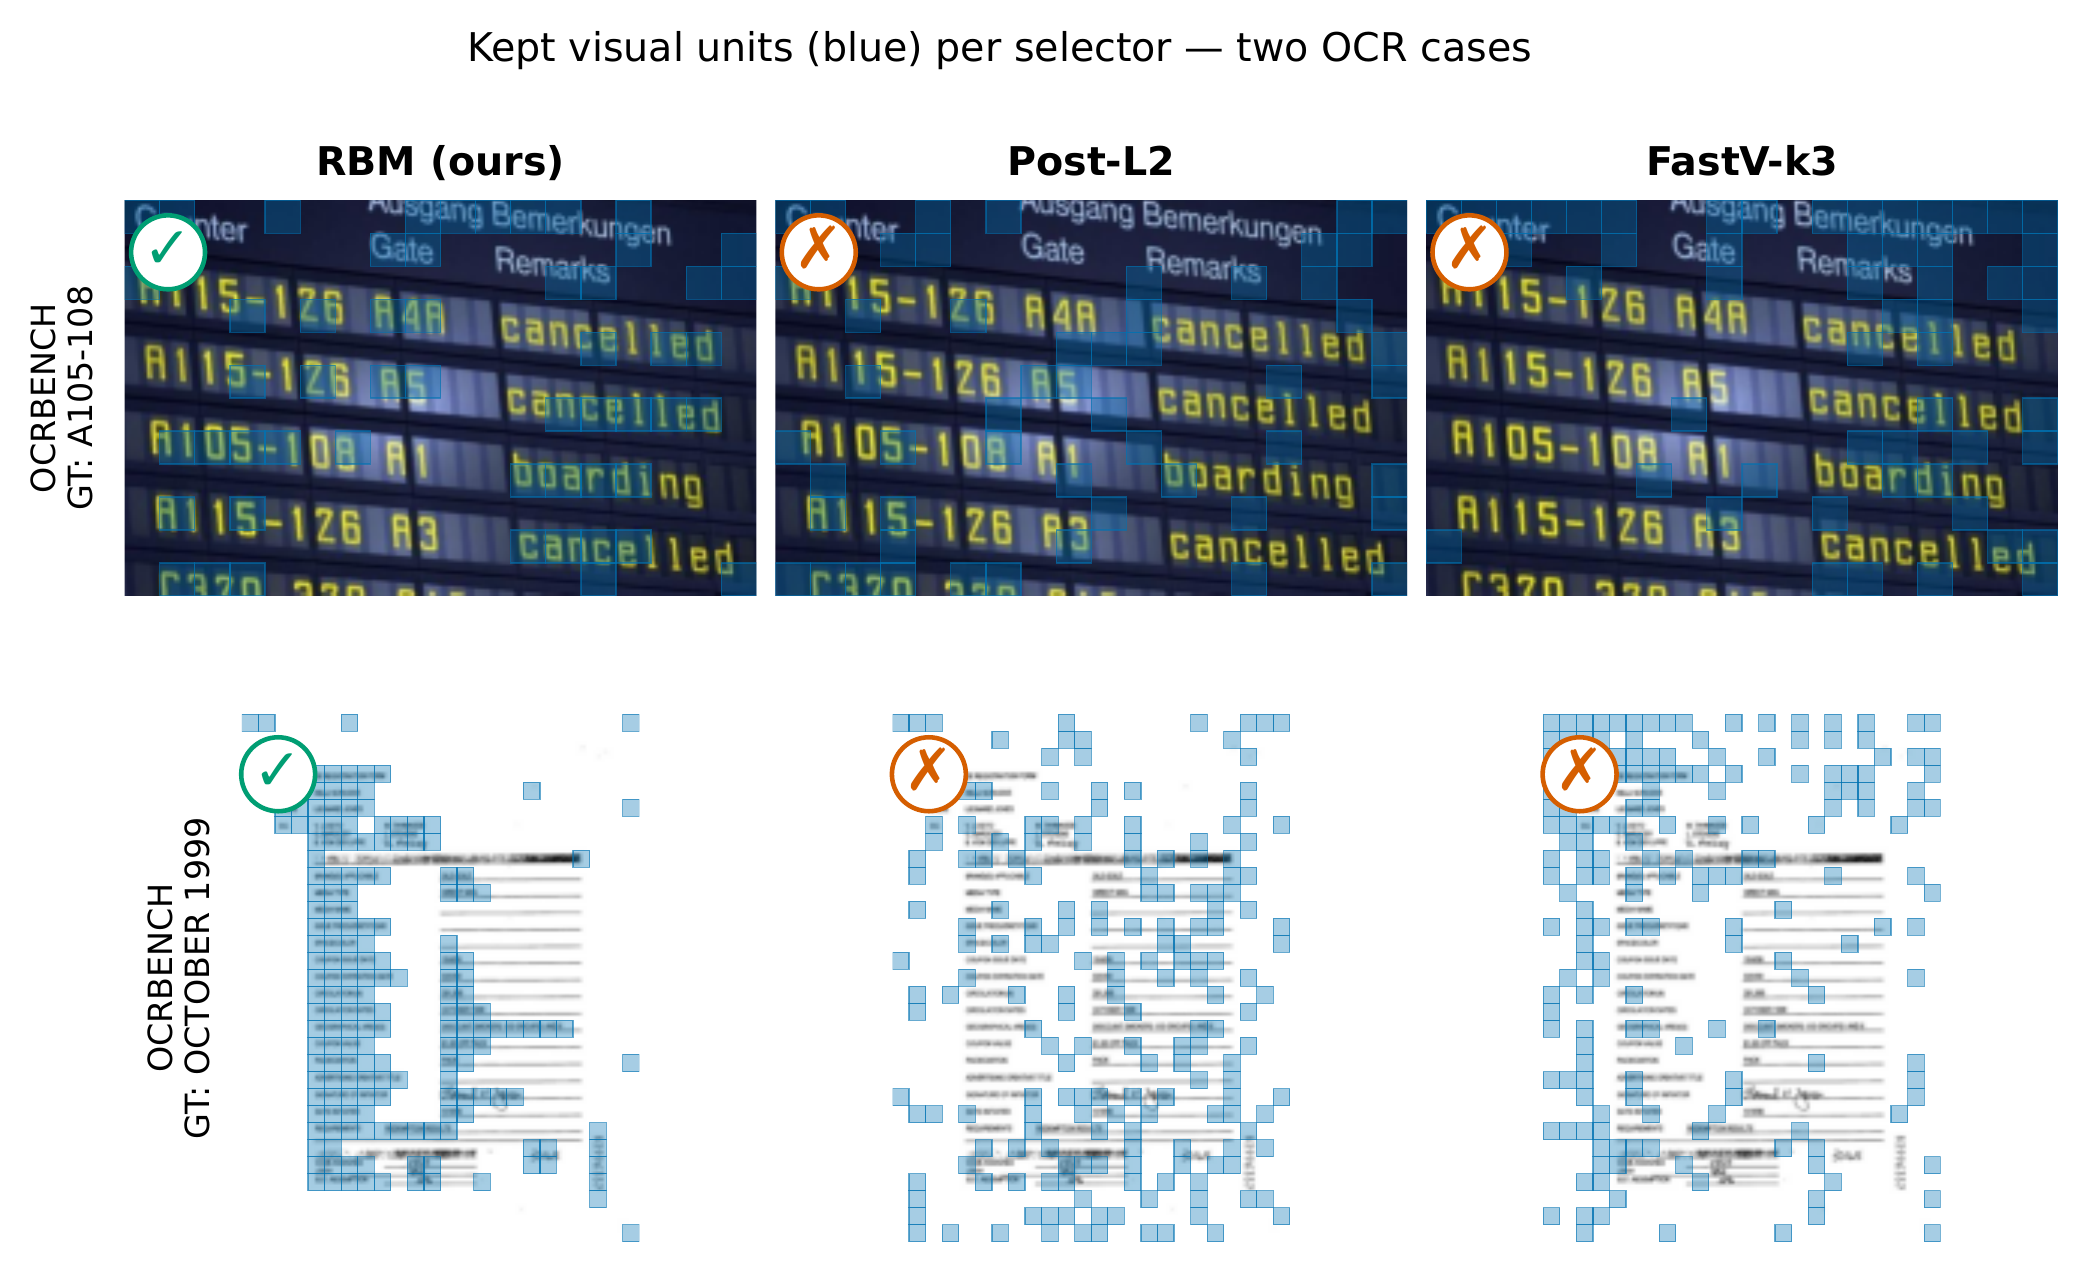
\includegraphics[width=.72\textwidth]{figs/fig2_word.png}
\caption{\label{fig:ocr-cases}Historical selected OCRBench cases at 25\% retention. Blue cells show recaptured retained-unit masks; checkmarks indicate correctness of the historical predictions under the official answer rule.}
\end{figure*}

The deployed RBM adapters exceed Post-L2 on all nine text-dense comparisons. The Qwen3-VL controls reveal a task-dependent pattern: final-input selection favors TextVQA and OCRBench, while main-output selection favors DocVQA and GQA. Under shared attention, FastV exceeds RBM on full TextVQA, while RBM exceeds FastV on OCRBench. RBM also exceeds Hi-Lo on TextVQA, with an OCRBench difference whose interval crosses zero. Our contributions are a native-unit norm selector integrated with three existing interfaces, full-split representation controls, and a Qwen3-VL evaluation of stronger selectors, retention curves, and complete-request costs.

\section{Related Work}
Visual-token reduction uses different signals and pruning locations. FastV and progressive methods remove tokens inside the language model using attention or layerwise decisions~\cite{chen2024fastv,xing2024pyramiddrop,zhang2024fastervlm,zhang2024sparsevlm}. Encoder-output methods instead use attention, graph propagation, fitted predictors, or combined cues~\cite{wang2024vtccls,shang2024prumerge,ye2024fitprune,jiang2025gprune,luan2025adaptprune}. Unified selectors combine saliency with diversity or text guidance~\cite{yu2026visiontrim,baek2026agilepruner,fang2026prunesid}. RBM uses an image-only norm score on complete native units at a merger or projector input.

Token merging also changes the representation used by a selector. ToMe, VisionZip, and AdaptMerge employ matching, dominant-token preservation, or language guidance~\cite{bolya2023tome,yang2024visionzip,islam2025adaptmerge}; TokenPacker learns a compact projector~\cite{li2024tokenpacker}. GlimpsePrune, VScan, and AnchorPrune adapt reduction to inputs or model families~\cite{zeng2025glimpseprune,zhang2025vscan,oh2026anchorprune}. RBM reuses an existing model's native operator and dimensions, selecting its input units rather than learning a new projection or synthesizing a new merged representation.

QuietPrune maps a textual query to a visual-domain [Q-CLS] token and ranks spatial $2\times2$ groups by mean query-to-visual attention inside the vision transformer, preserving compatibility with native merging~\cite{gao2026quietprune}. RBM uses image-only feature norms at native merger/projector inputs and introduces no query adapter. Its deployed paths retain the full vision-transformer computation.

Recent work varies the reduction stage and the information preserved by selection. PixelPrune, TransPrune, and V2Drop move pruning earlier or vary it across tokens and layers~\cite{wang2026pixelprune,li2026transprune,chen2026v2drop}. Hi-Lo Prune combines hierarchical candidate selection with information fusion before an early language-model pruning layer~\cite{sun2026hiloprune}; we evaluate its released Qwen3-VL image path. ApET, SCORE, COIN, ZOO-Prune, and SPARE use coverage, reconstruction, approximation, or sensitivity objectives~\cite{ma2026apet,xu2026score,du2026coin,kim2026zooprune,lee2026spare}. MetaCompress, EvoComp, IFPrune, and HAWK model semantics, information flow, or attention-head importance~\cite{wang2026metacompress,song2026evocomp,sun2026ifprune,zhu2026hawk}. Layer-dependent analysis identifies when pruning can be worse than random~\cite{wang2026informationhorizon}, while adaptive layerwise, pre-LLM text-driven, object-centered, local/global, and hybrid approaches vary the unit or context used for reduction~\cite{chen2026alvts,li2026crisp,lei2026core,li2026aot,zhang2026hybrid}. These approaches motivate evaluating the scoring representation together with the pruning stage and the model's native unit structure.

Document-focused pruning and provenance audits examine spatial evidence in text-dense inputs~\cite{choi2026docprune,liu2026provenance}, while EffiVLM-Bench and LMMs-Eval support systematic efficiency and accuracy evaluation~\cite{wang2025effivlmbench,zhang2024lmmseval}. We study Qwen2.5-VL, Qwen3-VL, and InternVL3~\cite{bai2025qwen25vl,bai2025qwen3vl,zhu2025internvl3}, whose native compression interfaces differ. Post-L2 provides a representation diagnostic from the same magnitude-based family; FastV and Hi-Lo supply stronger comparisons based on attention and hierarchical selection.

\section{Native-Unit Compression}
\subsection{Selection representation and token budget}
For each budgeted collection of $N$ native spatial units (an image or a tile), each unit groups four patch vectors. At retention $\rho$, retain
\begin{equation}
k=\max\{1,\operatorname{round}(\rho N)\}.
\end{equation}
For the Qwen adapters, features $h^{(t)}_{u,j}$ at tap $t$ give the unit score
\begin{equation}
a_u^{(t)}=\frac{1}{4}\sum_{j=1}^{4}\|h^{(t)}_{u,j}\|_2,
\qquad K_{\mathrm{RBM}}=\operatorname{TopK}_k\{a_u^{(t)}\}.
\label{eq:pre}
\end{equation}
InternVL3 scores the concatenated vector after pixel shuffle:
\begin{equation}
a_u^{(t)}=\left(\sum_{j=1}^{4}\|h^{(t)}_{u,j}\|_2^2\right)^{1/2}.
\label{eq:intern}
\end{equation}
Both implementations rank complete native units; their within-unit norm aggregation differs.

An output selector instead scores a returned visual vector $z_u$:
\begin{equation}
b_u=\|z_u\|_2,\qquad
K_{\mathrm{post}}=\operatorname{TopK}_k\{b_u\}.
\label{eq:post}
\end{equation}
Input and output norms can induce different top-$k$ sets. We measure selection disagreement with Jaccard overlap and evaluate its task-level consequences. For a fixed retained set, an independent per-unit merger returns the same retained representations whether units are gathered before or after that merger.

\subsection{Deployed adapters and controlled variants}
RBM retains complete units and aligns their identities with each adapter's output streams. Weights and interface dimensions are reused. For feature dimension $d$, norm scoring costs $O(Nd)$, followed by top-$k$ selection. Table~\ref{tab:adapters} specifies the deployed paths; their feature depth, aggregation, ordering, and allocation are part of the implementation comparison.

\begin{table*}[t]
\centering
\caption{\label{tab:adapters}Deployed adapter definitions. Post-L2 is the model-specific output-norm baseline. The Qwen3-VL main stream and three auxiliary deepstack streams share retained identities.}
\small
\begin{tabular}{@{}p{.13\textwidth}p{.25\textwidth}p{.24\textwidth}p{.29\textwidth}@{}}
\toprule
Model & RBM scoring representation & Post-L2 scoring representation & Allocation and sequence handling\\
\midrule
Qwen3-VL & Layer-8 deepstack input; mean of four patch norms & Concatenated main and three deepstack outputs & One per-image set, shared across four merger streams; adapter compressed positions\\
Qwen2.5-VL & Main-merger input; mean of four patch norms & Main-merger output & Per-image budget; pre/post ordering differs; vLLM assigns the first $k$ grid positions\\
InternVL3 & Post-pixel-shuffle input to projector; concatenated-vector norm & Post-projector vector & RBM budgets per tile; Post-L2 pools image tiles; adapter compressed positions\\
\bottomrule
\end{tabular}
\end{table*}

The Qwen3-VL controls compare four variants. Deployed RBM scores the early layer-8 input. \emph{Pre-final} scores final-block features at the main-merger input. \emph{Post-main} scores only the main-merger output. \emph{Post-concat}, the Qwen3-VL Post-L2 baseline, scores the concatenation of main and auxiliary outputs. The latter three variants execute every merger stream and match samples and per-image final counts. Pre-final versus Post-main compares four input-patch norms with the main-output norm; Post-main versus Post-concat changes the scored output streams. These definitions make the measured representation and aggregation choices explicit.

\section{Evaluation Protocol}
We evaluate Qwen3-VL-8B, Qwen2.5-VL-7B, and InternVL3-8B in bf16 with greedy decoding. The three-model matrix and final-input control use vLLM 0.19 V1~\cite{kwon2023vllm}. The additional Qwen3-VL selector, budget, and request-cost experiments use HuggingFace Transformers. We report the two frameworks in separate comparisons.

The full evaluation sets contain 5,000 TextVQA examples, 5,349 DocVQA examples, 1,000 OCRBench examples, and 12,578 GQA examples~\cite{singh2019textvqa,mathew2021docvqa,liu2024ocrbench,hudson2019gqa}. Saved predictions are rescored with pinned lmms-eval benchmark implementations~\cite{zhang2024lmmseval}. TextVQA uses answer normalization and leave-one-annotator-out consensus over the original ten-answer annotations. DocVQA uses ANLS with case and whitespace normalization and a 0.5 similarity threshold. OCRBench applies fullwidth-to-ASCII normalization and case-insensitive answer containment, with case-sensitive containment after removing spaces for handwritten mathematical expressions, and is scored out of 1,000. GQA uses exact match ignoring case and punctuation. The three former benchmarks are designated text-dense; GQA provides an object-centered question-answering contrast.

The three-model comparisons retain 25\% of native units and match per-image final counts. Qwen3-VL controls use native resolution, greedy decoding to 32 tokens, and vLLM eager execution; sequence limits are 8,192 with eight concurrent sequences, except DocVQA at 32,768 and four. The operational compressed arms and final-input controls complete every sample. Uncompressed TextVQA anchors have two failures for each Qwen model, and the Qwen3-VL OCRBench anchor has 18; these failures receive zero. Qwen2.5-VL OCRBench and InternVL3 DocVQA use four-million-pixel caps, precluding absolute cross-family ranking.

Control-comparison 95\% intervals use 20,000 paired-bootstrap resamples of per-example scores. Failed samples receive zero in complete-split scores and their paired analyses.

\subsection{Additional Qwen3-VL selector and budget protocol}
The additional experiments fix Qwen3-VL-8B-Instruct weights, Transformers 4.57.6, PyTorch 2.10.0, bf16, native spatial positions, batch size one, seed 0, and greedy decoding capped at 32 tokens. The primary full-split comparison and request-cost workload use SDPA in the vision encoder and eager attention in the language model for every arm (Table~\ref{tab:hfprotocols}). They share a four-million-pixel cap, input processing, prompts, and per-image final counts at each compressed budget. None retains all visual units.

Hi-Lo uses the authors' Qwen3-VL implementation at commit \texttt{29265e3}, with a configuration-compatibility shim and removal of a type-conversion block whose guard references an undefined variable. Its hierarchical selection and fusion are retained. This vendored model path remains different from the standard HuggingFace implementation used by None, RBM, and FastV.

Hi-Lo prunes at layer index 2, after the three deepstack injections, with fusion strength .3, top-$k$ ratio .1, and attention threshold .05. FastV-k3 uses zero-based pruning index 3, so its first four decoder-layer inputs retain all visual tokens. The Hi-Lo candidate fraction is $\max(.30,\rho)$ to satisfy the official candidate-count constraint; candidate and retained sets coincide at 50/75\%, leaving no separate candidate pool for fusion. Parameters are fixed before evaluation. Under shared attention, a no-pruning, fusion-disabled check on 32 fixed TextVQA requests gives identical native and vendored input-ID and position tensors, main/deepstack embeddings, first-token logits, and complete greedy token sequences. Separate eager keep-all checks match native greedy sequences on 32 TextVQA examples in each RBM/Post-L2/FastV path, with bf16 first-step logit differences up to .125. These are finite integration checks on the stated inputs.

The primary endpoints are 25\% retention on full TextVQA ($n=5{,}000$) and OCRBench ($n=1{,}000$), newly evaluated under the shared attention settings. The earlier retention curves use a seed-20261025 TextVQA subset of 1,000 examples, stratified by the recorded 25\%-retained unit count as a proxy for original unit count, and all 1,000 OCRBench examples. These curves retain their original mixed attention protocol: eager vision and language attention for None/RBM/FastV, and SDPA for Hi-Lo. Their saved 25\% RBM/FastV predictions are reused after configuration and sample-ID checks. The 500-example DocVQA stress test is stratified by image area and uses the same mixed attention settings, with a shared two-million-pixel cap selected after higher-resolution smoke tests exhausted memory. It remains separate from both the new full-split comparison and the historical vLLM DocVQA results. All attempted IDs remain in the denominator, with failed samples scored zero. Common-completion analyses expose differences in failure coverage.

\begin{table*}[t]
\centering
\caption{\label{tab:hfprotocols}HuggingFace protocol blocks. Shared attention denotes vision SDPA and language-model eager attention for all methods. Mixed attention denotes eager/eager for None, RBM, and FastV, and SDPA/SDPA for Hi-Lo. Hi-Lo uses the authors' adapted model in every block. Listed retention rates apply to compressed arms; None retains 100\%. Quality and cost are paired only within the same protocol and sample IDs.}
\small
\begin{tabular}{@{}lllll@{}}
\toprule
Block & Examples & Attention & Pixel cap & Retention\\
\midrule
Primary full-split comparison & TextVQA 5,000; OCRBench 1,000 & Shared & 4M & 25\%\\
Quality--cost workload & TextVQA 100; OCRBench 100 & Shared & 4M & 25/50/75\%\\
Retention curves & TextVQA 1,000; OCRBench 1,000 & Mixed & 4M & 25/50/75\%\\
DocVQA stress test & DocVQA 500 & Mixed & 2M & 25\%\\
\bottomrule
\end{tabular}
\end{table*}

\section{Results}
\subsection{Operational accuracy across model families}
Table~\ref{tab:main} compares deployed RBM with Post-L2. Across the six TextVQA/DocVQA cells, RBM gains 11.0--38.0 percentage points; the three OCRBench gains are 298--432 points out of 1,000. On Qwen3-VL DocVQA, RBM scores .481 compared with .956 without compression.

\begin{table*}[t]
\centering
\caption{\label{tab:main}Full-split operational results at 25\% retention. None denotes no compression. Qwen3-VL RBM uses the early tap. Deltas use unrounded scores and are percentage points except for OCRBench (/1000).}
\small
\setlength{\tabcolsep}{4pt}
\begin{tabular}{llrrrr}
\toprule
Model & Benchmark & None & RBM & Post-L2 & $\Delta$\\
\midrule
\multirow{4}{*}{Qwen3-VL}
& TextVQA & .8343 & .5978 & .2181 & +38.0\\
& DocVQA & .9563 & .4809 & .2378 & +24.3\\
& OCRBench & 760 & 547 & 184 & +363\\
& GQA & .6165 & .4486 & .4769 & $-2.8$\\
\midrule
\multirow{4}{*}{Qwen2.5-VL}
& TextVQA & .8529 & .6941 & .4360 & +25.8\\
& DocVQA & .9492 & .6361 & .5258 & +11.0\\
& OCRBench & 817 & 480 & 182 & +298\\
& GQA & .6045 & .5571 & .5852 & $-2.8$\\
\midrule
\multirow{4}{*}{InternVL3}
& TextVQA & .8251 & .7804 & .4093 & +37.1\\
& DocVQA & .9223 & .7285 & .3820 & +34.6\\
& OCRBench & 852 & 753 & 321 & +432\\
& GQA & .6287 & .5985 & .6028 & $-0.4$\\
\bottomrule
\end{tabular}
\end{table*}

GQA favors Post-L2 in all three point estimates. The small InternVL3 difference has an interval crossing zero in the paired analysis. Thus, the operational advantage on text-dense tasks does not extend to the object-centered GQA workload.

\subsection{Input representation and output-stream aggregation}
Table~\ref{tab:stage} compares final-input selection with the two output selectors. Changing Post-concat to Post-main raises DocVQA from .2378 to .3737, reversing its relation to Pre-final (.2837). Post-main exceeds Pre-final by 9.00 percentage points on DocVQA and 6.19 points on GQA; Pre-final leads by 17.94 percentage points on TextVQA and 63 points on OCRBench. The direction of input-versus-output selection therefore depends on the task and the scored streams.

\begin{table*}[t]
\centering
\caption{\label{tab:stage}Qwen3-VL full-split controls at 25\% retention. Pre-final scores the main-merger input; Post-main scores its output; Post-concat scores the concatenated main-plus-deepstack output. Differences and paired-bootstrap 95\% intervals are percentage points, except OCRBench points out of 1,000.}
\small
\begin{tabular}{lrrrll}
\toprule
Benchmark & Pre-final & Post-main & Post-concat & Main $-$ Pre [95\% CI] & Pre $-$ Concat [95\% CI]\\
\midrule
TextVQA & .4917 & .3123 & .2181 & $-17.94$ [$-19.45$, $-16.45$] & +27.36 [25.88, 28.81]\\
DocVQA & .2837 & .3737 & .2378 & +9.00 [7.82, 10.17] & +4.59 [3.41, 5.77]\\
OCRBench & 419 & 356 & 184 & $-63$ [$-100$, $-27$] & +235 [200, 271]\\
GQA & .4198 & .4816 & .4769 & +6.19 [5.43, 6.96] & $-5.72$ [$-6.50$, $-4.92$]\\
\bottomrule
\end{tabular}
\end{table*}

\subsection{Comparison with stronger selectors}
Table~\ref{tab:fastv} compares None, RBM, FastV-k3, and the official Hi-Lo adaptation under shared vision SDPA and language-model eager attention. All methods use the same input processing, four-million-pixel cap, native positions, and decoding settings. Compressed arms match actual per-image final visual counts at 25\% retention. Scores use every attempted example, with failures assigned zero; paired-bootstrap intervals compare predictions on the same IDs.

Every method completes all 5,000 TextVQA and 1,000 OCRBench inputs without failure. Input hashes, original visual counts, full prompt lengths, and compressed per-image budgets match across methods. On TextVQA, RBM scores 75.58\%, compared with FastV's 76.90\% and Hi-Lo's 66.75\%. RBM minus FastV is $-1.32$ percentage points [$-2.32$, $-.34$]; RBM minus Hi-Lo is +8.83 [7.63, 10.04]. All three compressed arms remain below the uncompressed 83.45\% reference.

On OCRBench, RBM scores 610 versus FastV's 453, a difference of +157 points out of 1,000 [128, 187]. Hi-Lo scores 612; RBM minus Hi-Lo is $-2$ [$-31$, 27], whose interval crosses zero. This comparison does not establish equivalence. All compressed arms remain below the uncompressed score of 765. Thus, the relative ranking depends on the task even with attention settings and final token counts matched.

A separate historical Qwen2.5-VL eager comparison gives RBM 382 versus FastV 295 on OCRBench, with 88 shared failures and a paired difference of 87 points [54, 120]. Figure~\ref{fig:ocr-cases} shows selected OCRBench examples.

\begin{table*}[t]
\centering
\caption{\label{tab:fastv}Qwen3-VL full-split comparison under shared vision SDPA and language-model eager attention. Compressed arms retain 25\%; None is uncompressed. TextVQA reports accuracy percentages, and OCRBench reports points out of 1,000. Every method completes all inputs. The Hi-Lo adaptation uses the authors' model path.}
\small
\begin{tabular}{lrrrrr}
\toprule
Benchmark and unit & None & RBM & FastV-k3 & Hi-Lo & Per-arm completion\\
\midrule
TextVQA accuracy (\%) & 83.45 & 75.58 & 76.90 & 66.75 & $5{,}000/5{,}000$\\
OCRBench (points/1000) & 765 & 610 & 453 & 612 & $1{,}000/1{,}000$\\
\bottomrule
\end{tabular}
\end{table*}

\subsection{Retention curves and document stress test}
Table~\ref{tab:budgets} and Figure~\ref{fig:budgets} hold examples fixed across the three budgets under the mixed attention protocol. On the TextVQA subset, FastV has the highest point estimate at every budget, and all three methods improve as more units are retained. RBM's gap to its None reference decreases from 7.64 percentage points at 25\% retention to 1.20 points at 75\%. OCRBench also improves with retention. Its eager arms fail on 79 shared inputs, whereas Hi-Lo's SDPA path completes all 1,000. RBM and Hi-Lo have close point estimates on the fixed 921 commonly completed examples, while their complete-split difference includes failure coverage. At 25\%, Hi-Lo minus RBM on common examples is $-0.33$ percentage points [$-3.37$, 2.61].

We define a quality target as at least 95\% of the reported None reference within this mixed-attention block and consider only measured budgets. On the TextVQA subset, the first qualifying budget is 50\% for RBM and FastV, and 75\% for Hi-Lo. On attempted OCRBench scores, RBM and FastV first qualify at 75\%, and Hi-Lo at 50\%. Restricting OCRBench to the common 921 examples instead gives 75\% for all three methods. These are discrete quality thresholds; selecting the lowest-cost qualifying point additionally requires measured request cost under the same execution protocol.

\begin{table*}[t]
\centering
\caption{\label{tab:budgets}Qwen3-VL retention curves under the mixed attention protocol (Table~\ref{tab:hfprotocols}). TextVQA uses official accuracy (\%). Full OCRBench uses points out of 1,000, and its fixed common-921 sensitivity is normalized to 1,000. None scores are 82.93, 707, and 767.64 in the three blocks.}
\small
\begin{tabular}{llrrr}
\toprule
Benchmark & Retention & RBM & FastV & Hi-Lo\\
\midrule
\multirow{3}{*}{TextVQA subset ($n=1{,}000$)}
& 25\% & 75.29 & 76.95 & 66.20\\
& 50\% & 79.65 & 82.24 & 75.64\\
& 75\% & 81.73 & 82.57 & 81.24\\
\midrule
\multirow{3}{*}{OCRBench full split ($n=1{,}000$)}
& 25\% & 559 & 413 & 613\\
& 50\% & 659 & 569 & 709\\
& 75\% & 684 & 676 & 740\\
\midrule
\multirow{3}{*}{OCRBench common subset ($n=921$)}
& 25\% & 606.95 & 448.43 & 603.69\\
& 50\% & 715.53 & 617.81 & 711.18\\
& 75\% & 742.67 & 733.98 & 741.59\\
\bottomrule
\end{tabular}
\end{table*}

\begin{figure*}[t]
\centering
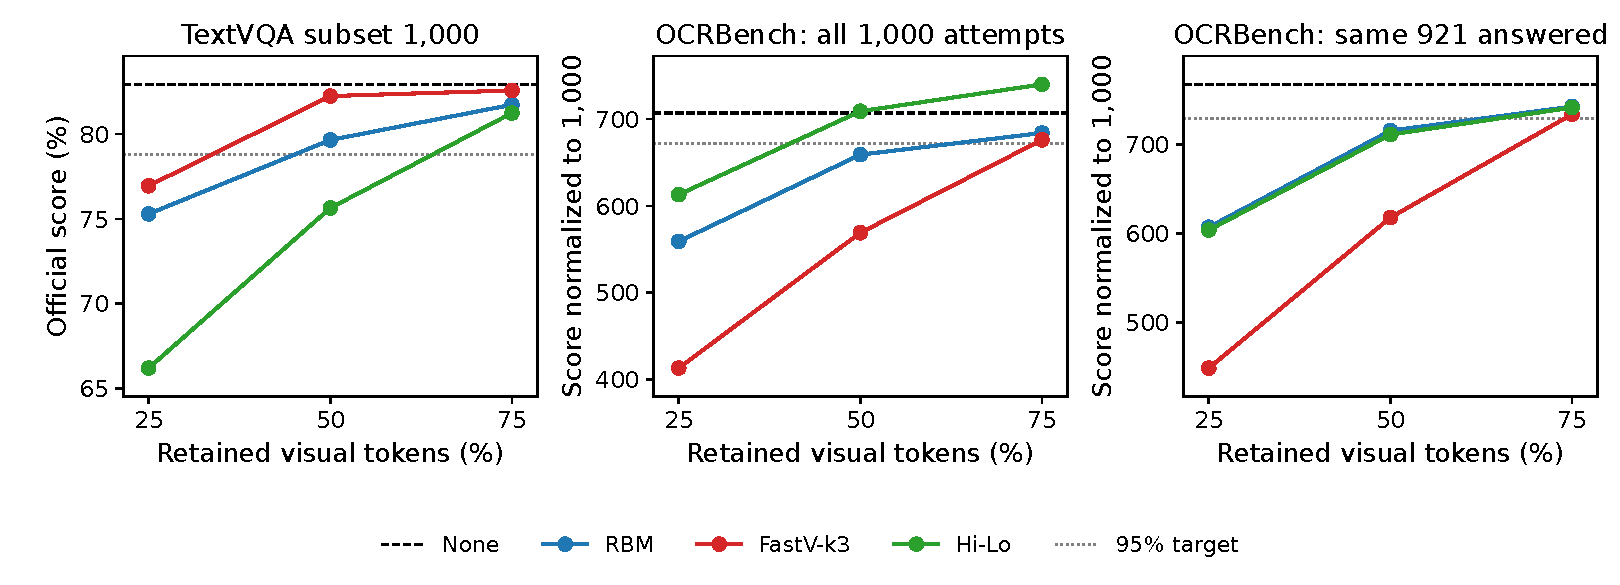
\includegraphics[width=\textwidth]{figs/budget_curves.pdf}
\caption{\label{fig:budgets}Qwen3-VL retention curves under the mixed attention protocol. TextVQA uses a fixed 1,000-example subset. OCRBench shows all 1,000 attempted examples and the fixed 921 examples completed by every method, revealing the effect of different failure coverage. Dashed lines mark uncompressed references; dotted lines mark their 95\% quality targets.}
\end{figure*}

The DocVQA stress test (Table~\ref{tab:docstress}) uses the mixed attention protocol, a unified two-million-pixel cap, and completes all 500 examples in every arm. At 25\% retention, RBM exceeds Hi-Lo by 6.39 percentage points [3.04, 9.78] and FastV by 12.32 points [8.15, 16.47]. The 500 questions cover 417 original document pages; 20,000 paired page-cluster bootstrap resamples, keeping each page's questions together, give intervals of [2.91, 9.87] and [8.05, 16.61] for the same differences. The result adds a document workload where RBM outperforms both stronger selectors, while its 12.96-point loss to None means that no compressed arm reaches the 95\% quality target. This subset result and the full-split representation controls address different protocols and comparisons.

\begin{table*}[t]
\centering
\caption{\label{tab:docstress}DocVQA stress test under the mixed attention protocol: fixed 500-example subset, two-million-pixel cap for all arms, and 25\% retention for compressed arms. All examples complete. ANLS and paired-bootstrap differences are in percentage points.}
\small
\begin{tabular}{lrrl}
\toprule
Method & Retention & ANLS (\%) & Difference from None [95\% CI]\\
\midrule
None & 100\% & 95.73 & ---\\
RBM & 25\% & 82.76 & $-12.96$ [$-15.96$, $-10.05$]\\
FastV-k3 & 25\% & 70.45 & $-25.28$ [$-28.97$, $-21.67$]\\
Hi-Lo & 25\% & 76.38 & $-19.35$ [$-22.76$, $-16.03$]\\
\bottomrule
\end{tabular}
\end{table*}

\section{Diagnostics and Interpretation}
The two operational Qwen3-VL rankings differ substantially. On 64 diagnostic images per benchmark, sampled with seed 0 from the corresponding 200-example subsets, DocVQA, TextVQA, and GQA Spearman correlations are .137, .332, and .360, and top-25\% Jaccard overlaps are .180, .243, and .278. These measurements quantify the selection disagreement between the deployed representations.

Rank shifts also associate with local edge energy: post-minus-pre rank correlations with Sobel energy are +.439, +.155, and +.036 in the same task order. On DocVQA, RBM-only versus Post-L2-only units have mean energy .641 versus .124, and 92\% versus 35\% exceed their image's median. Sobel energy measures local edges; we use it to characterize spatial selection rather than text localization. Figure~\ref{fig:survival} visualizes the spatial allocation in two audited cases.

\begin{figure*}[t]
\centering
% Viewports retain the original six data panels, with no changes to their marks.
% Original PDF size: 1131.13 x 855.60 bp. Coordinates are PDF bottom-left.
\begin{tabular}{@{}ccc@{}}
\multicolumn{3}{c}{\textbf{TextVQA 35174: 120 of 480 native units retained}}\\[3pt]
RBM & Post-L2 & Kept-set overlap\\[2pt]
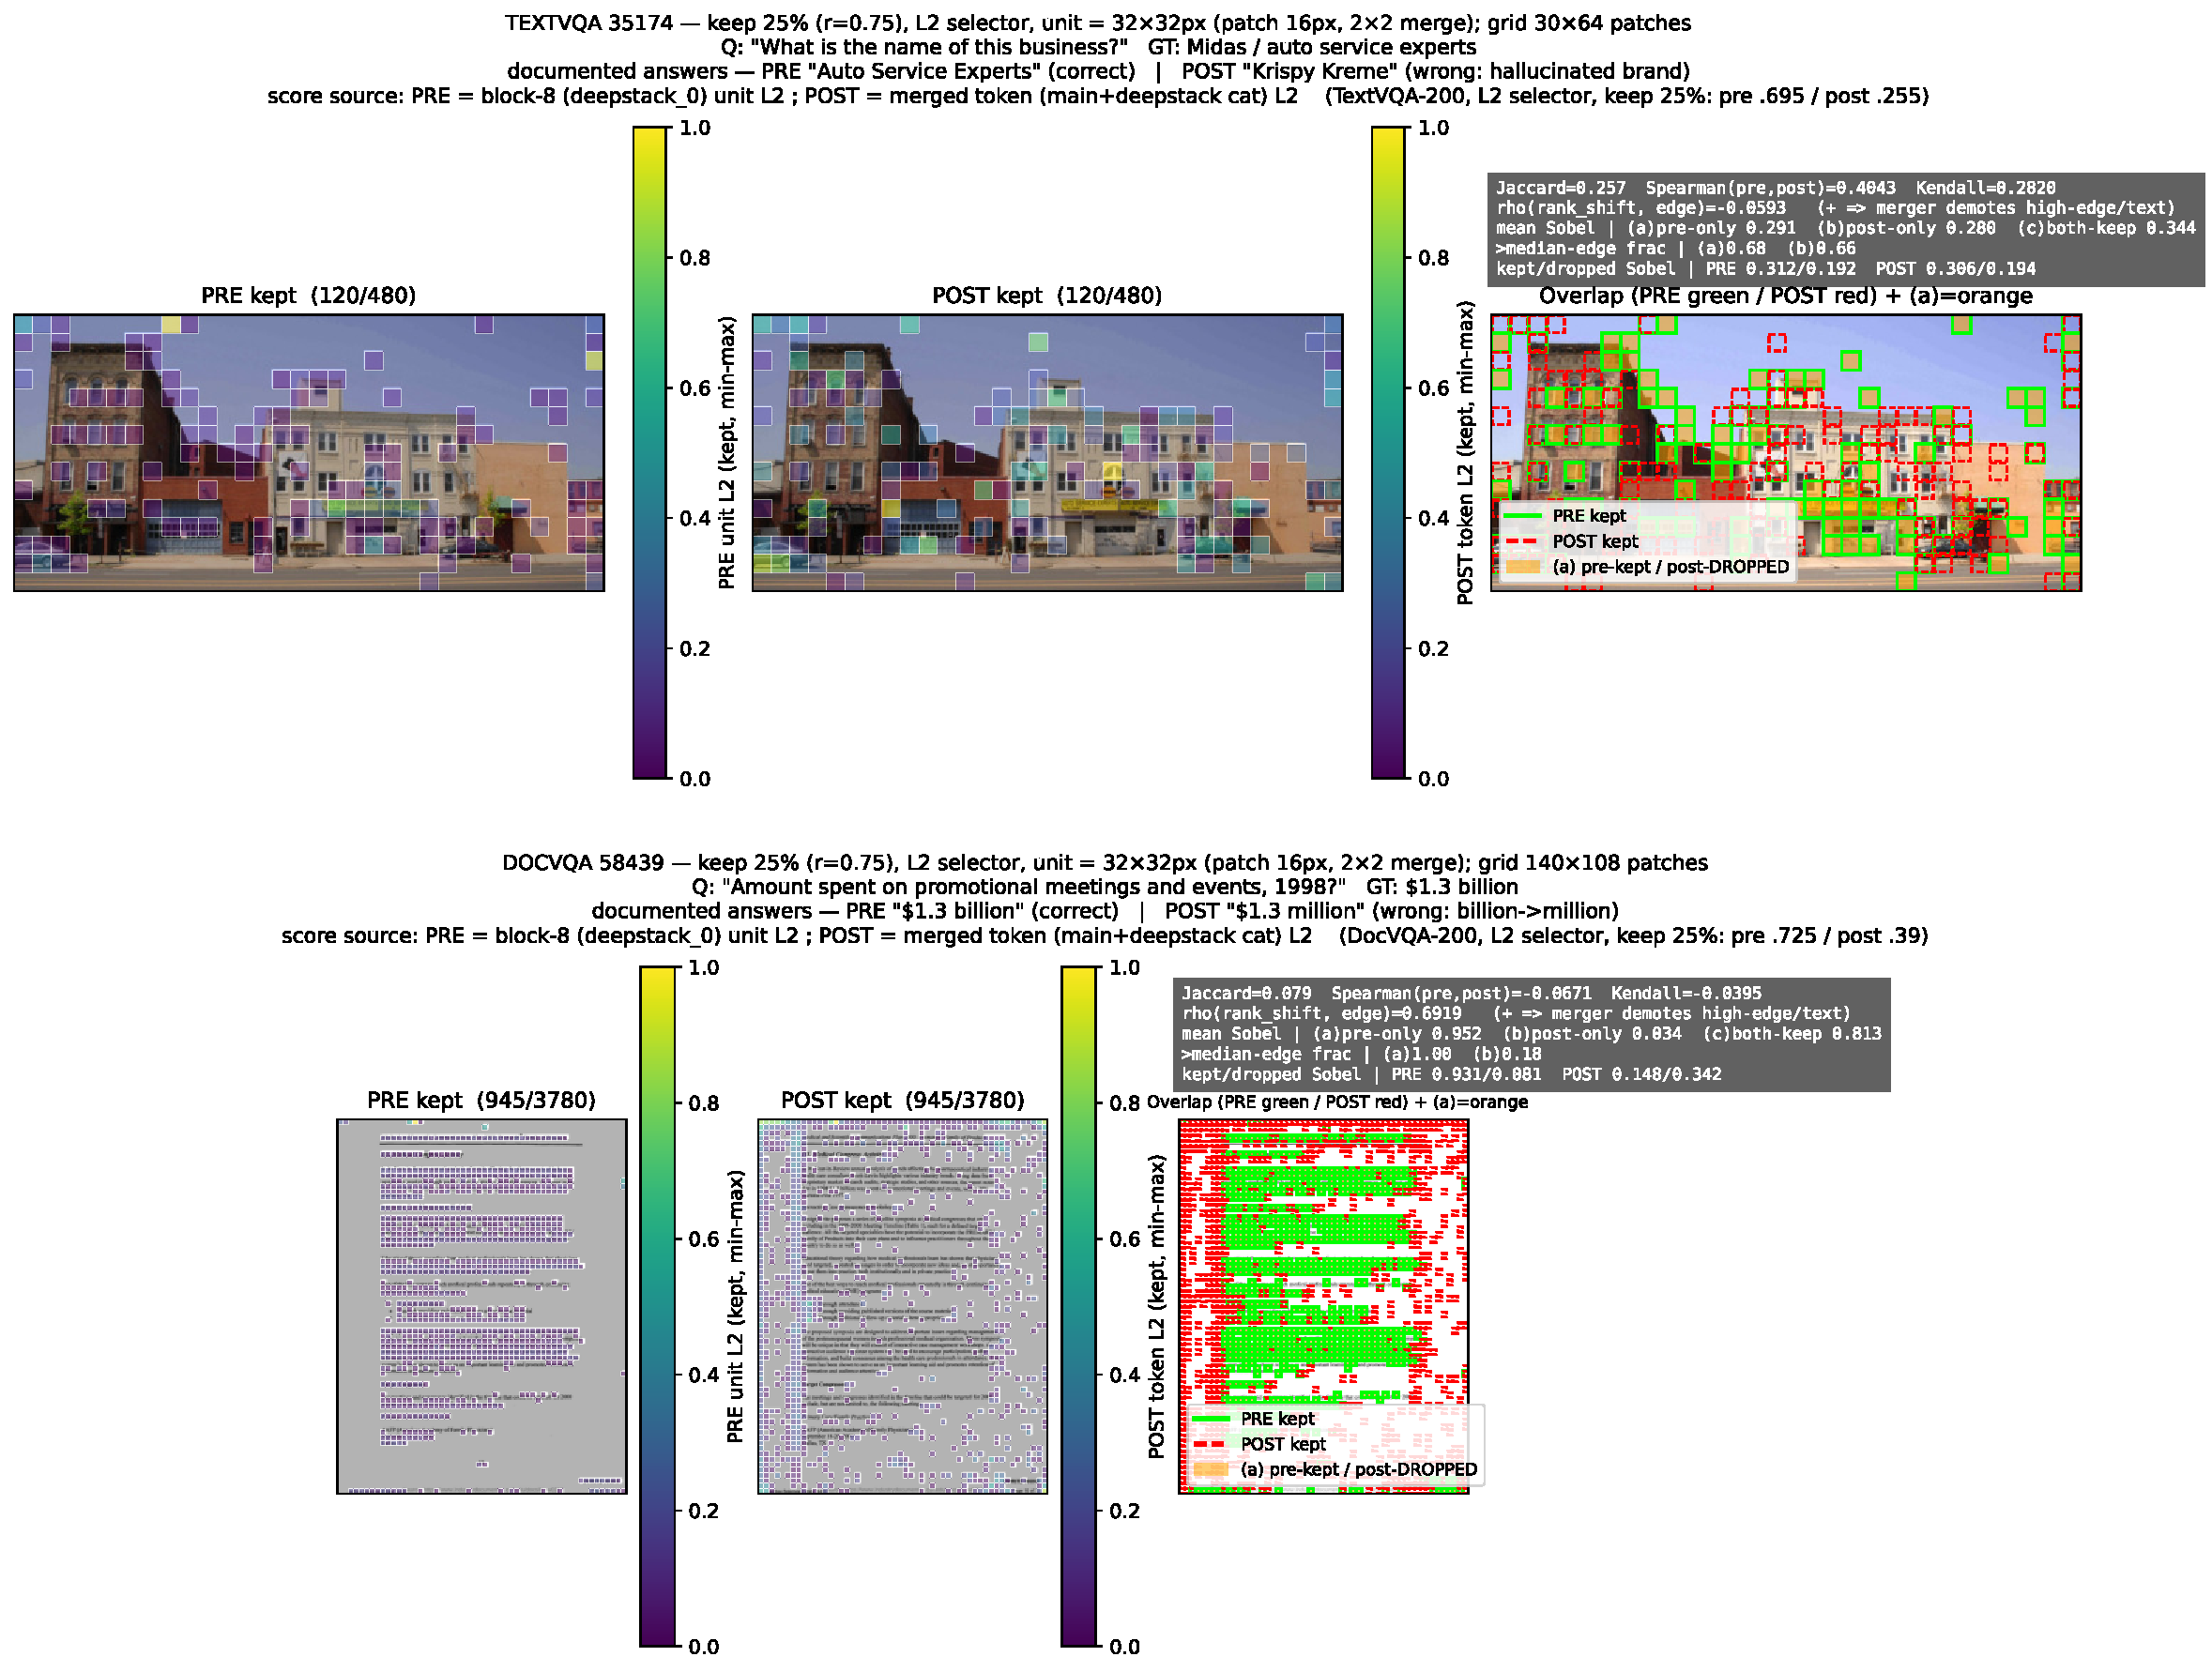
\includegraphics[viewport=6 552 310 695,clip,width=.31\textwidth]{figs/fig4_vector.pdf} &
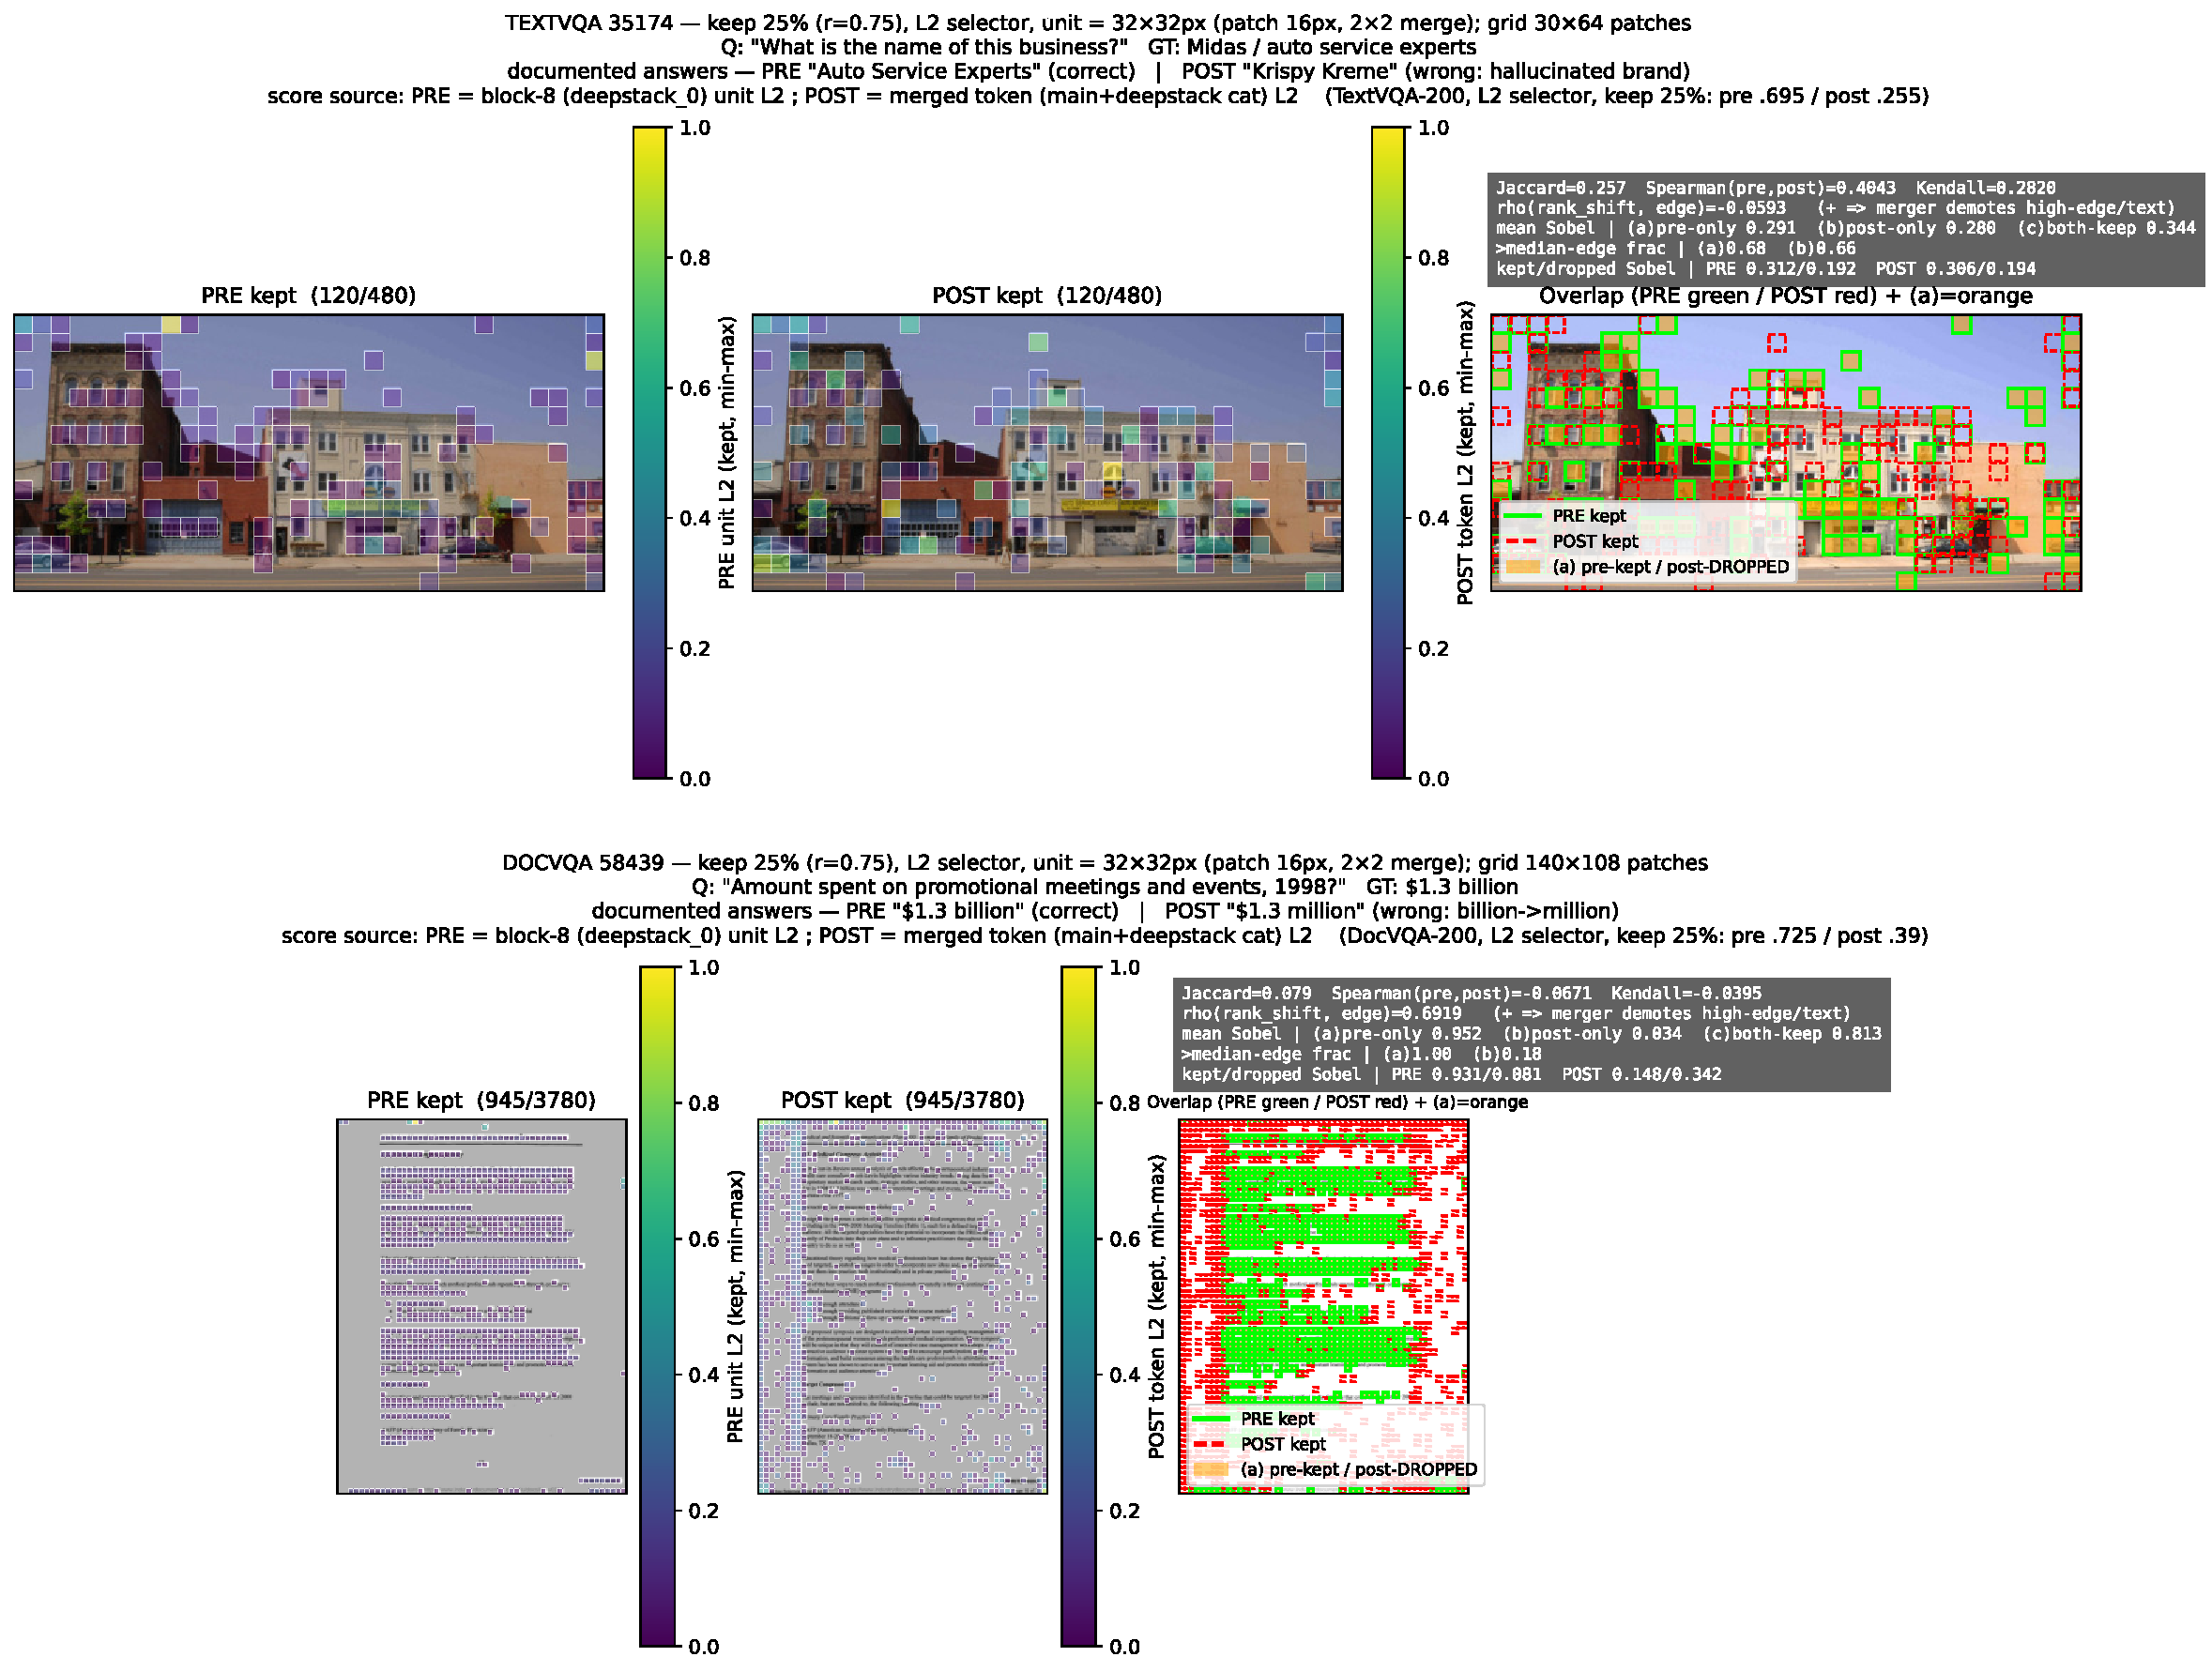
\includegraphics[viewport=384 552 688 695,clip,width=.31\textwidth]{figs/fig4_vector.pdf} &
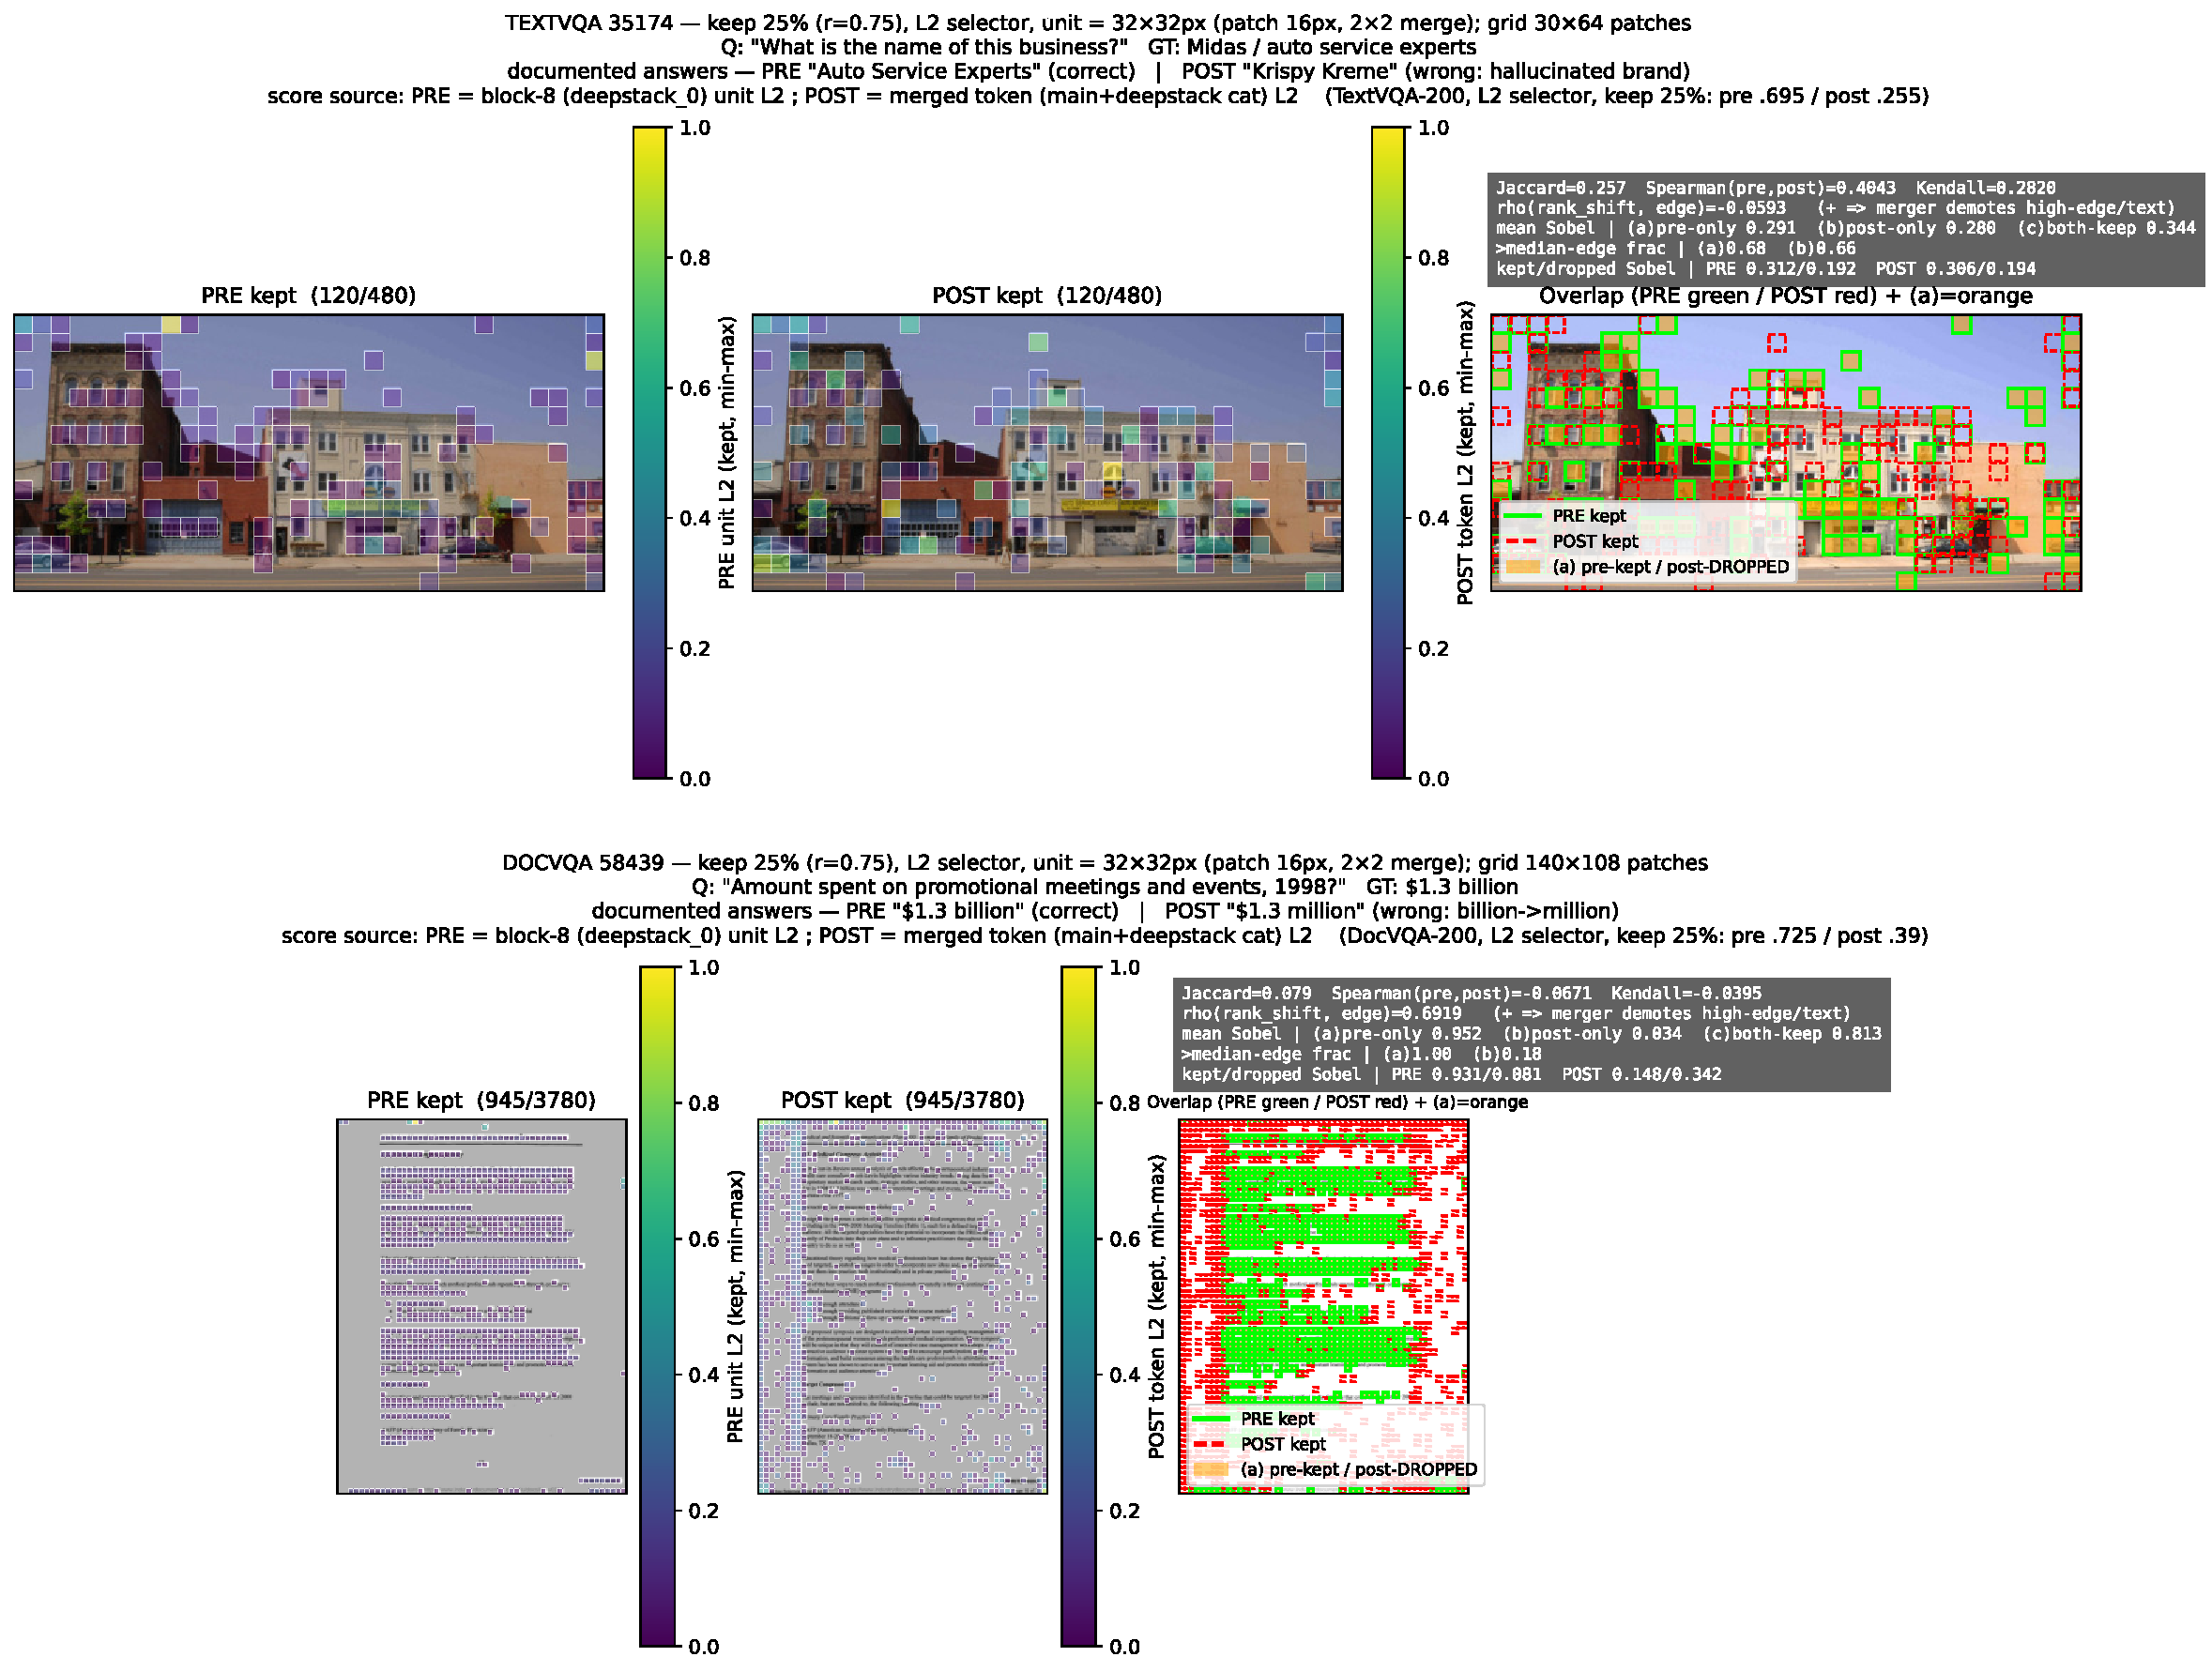
\includegraphics[viewport=762 552 1066 695,clip,width=.31\textwidth]{figs/fig4_vector.pdf}\\[8pt]
\multicolumn{3}{c}{\textbf{DocVQA 58439: 945 of 3,780 native units retained}}\\[3pt]
RBM & Post-L2 & Kept-set overlap\\[2pt]
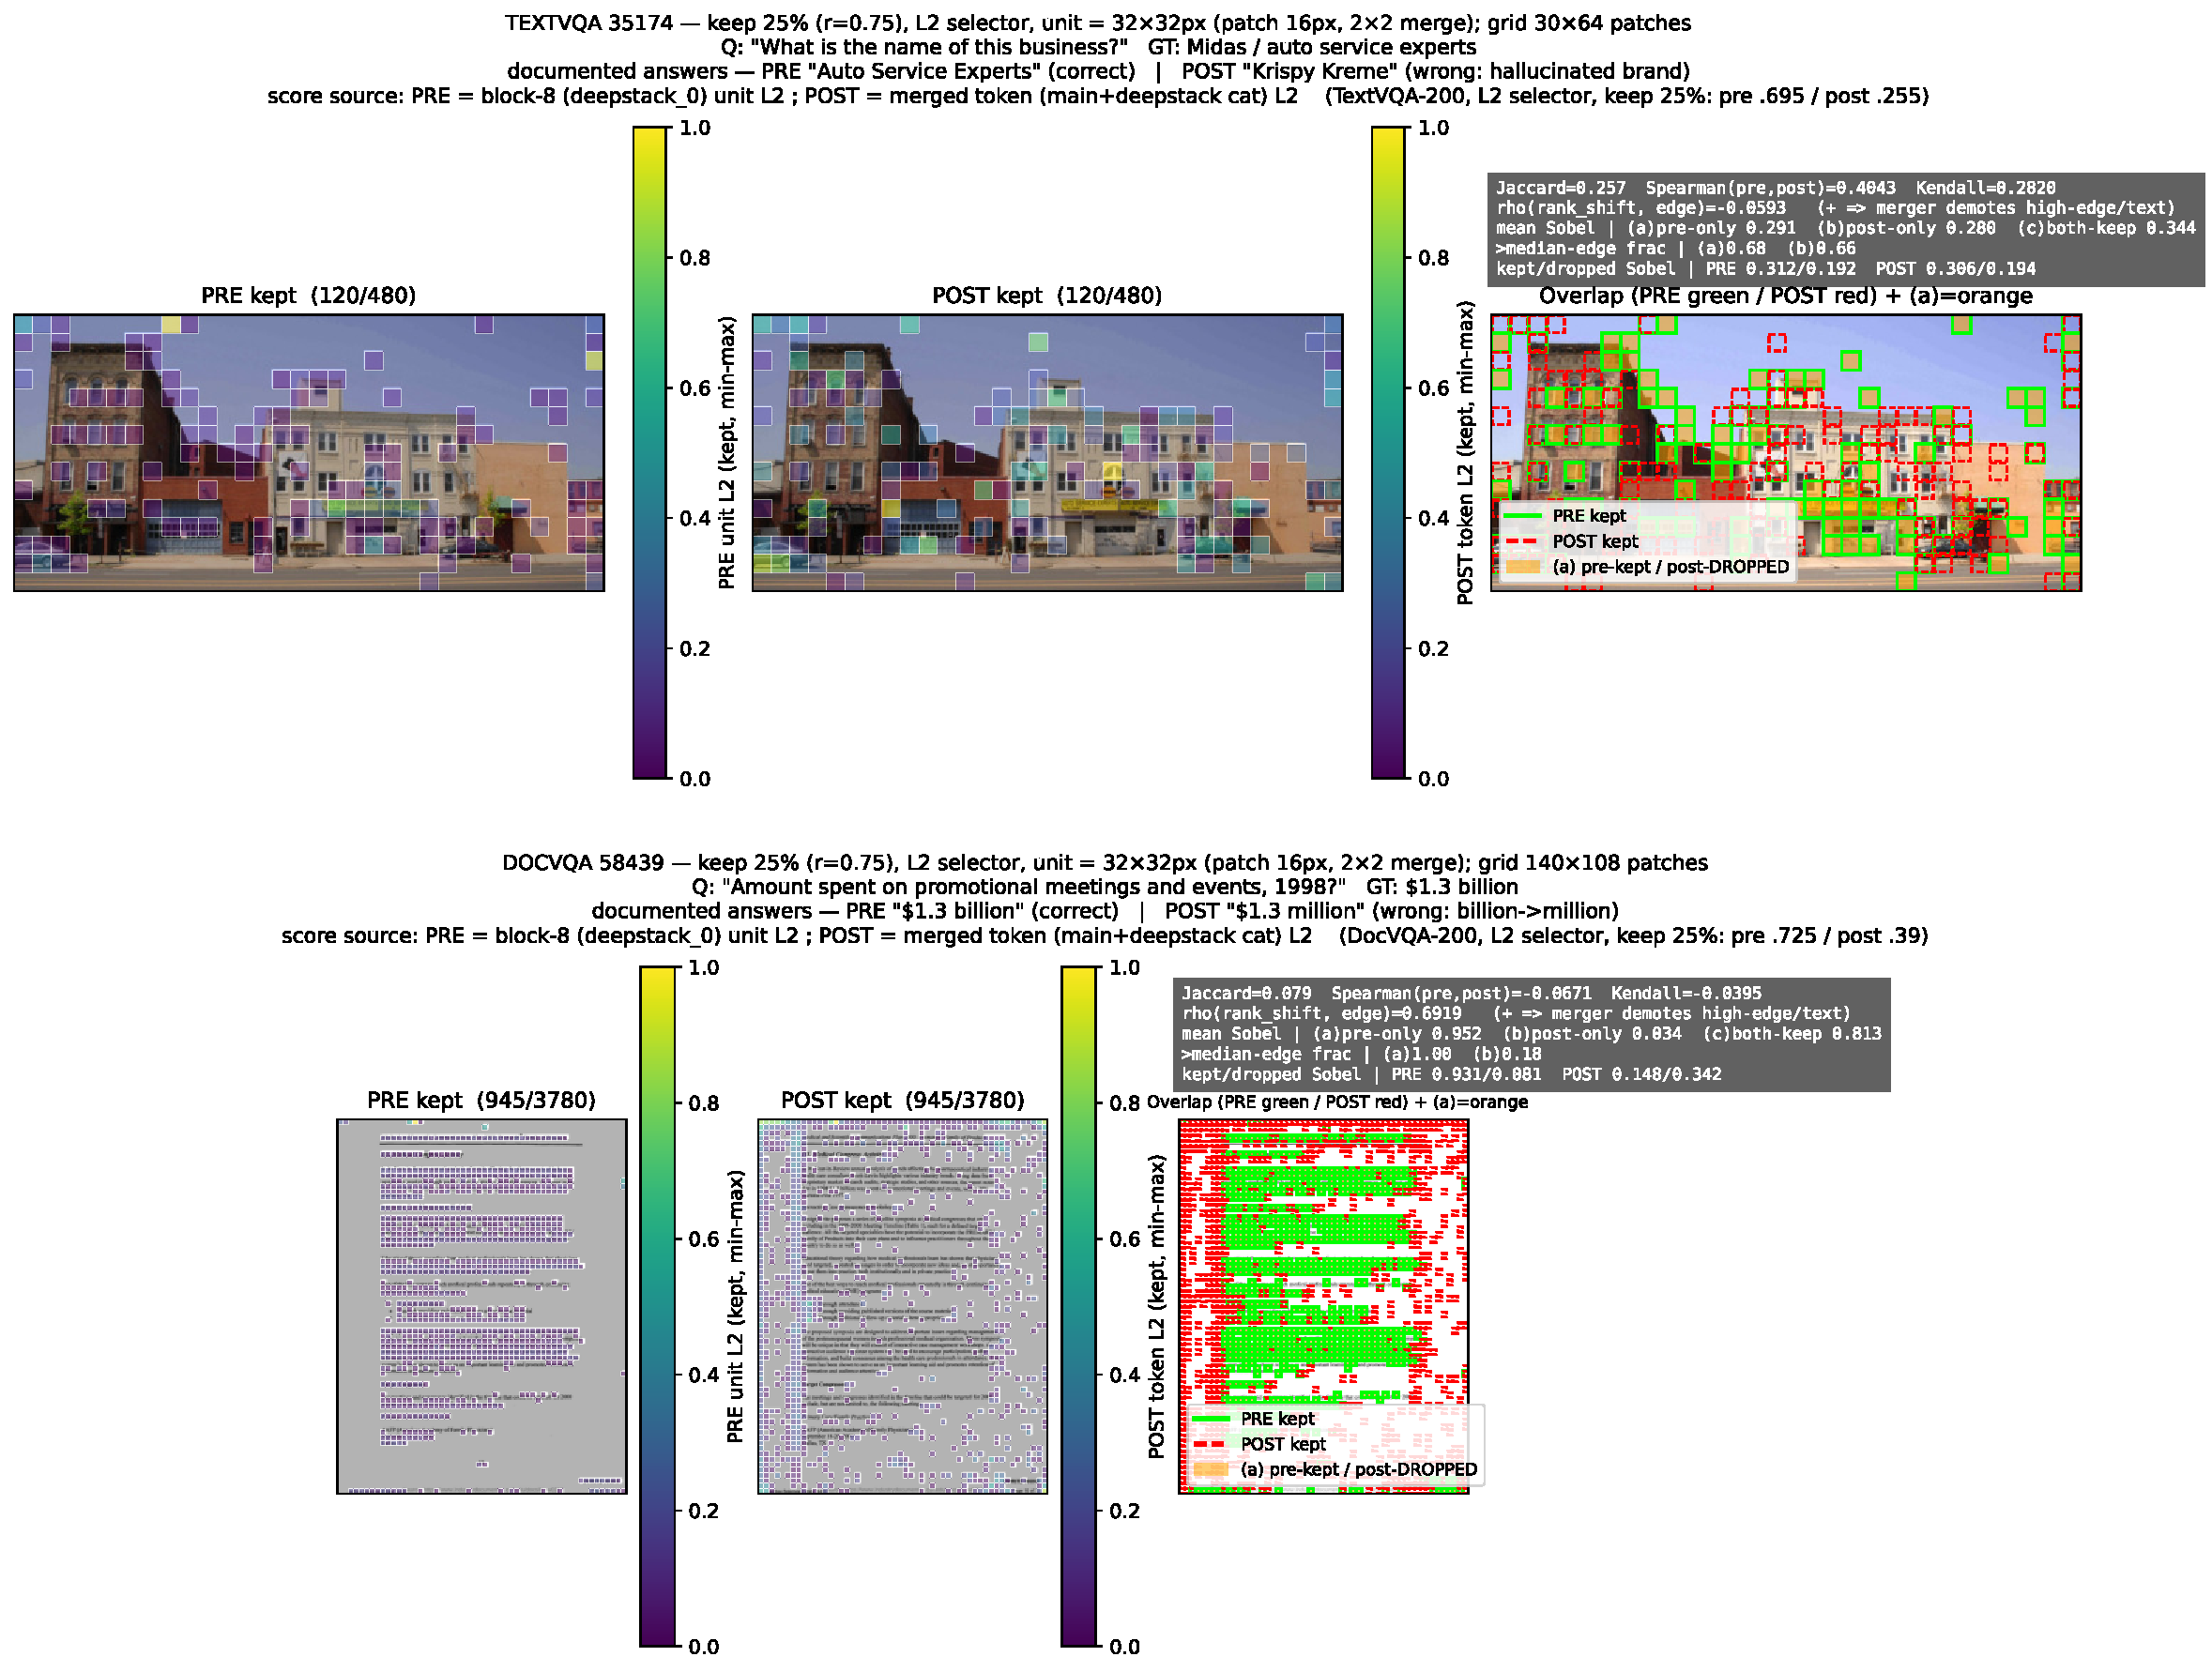
\includegraphics[viewport=171 90 321 283,clip,height=1.65in]{figs/fig4_vector.pdf} &
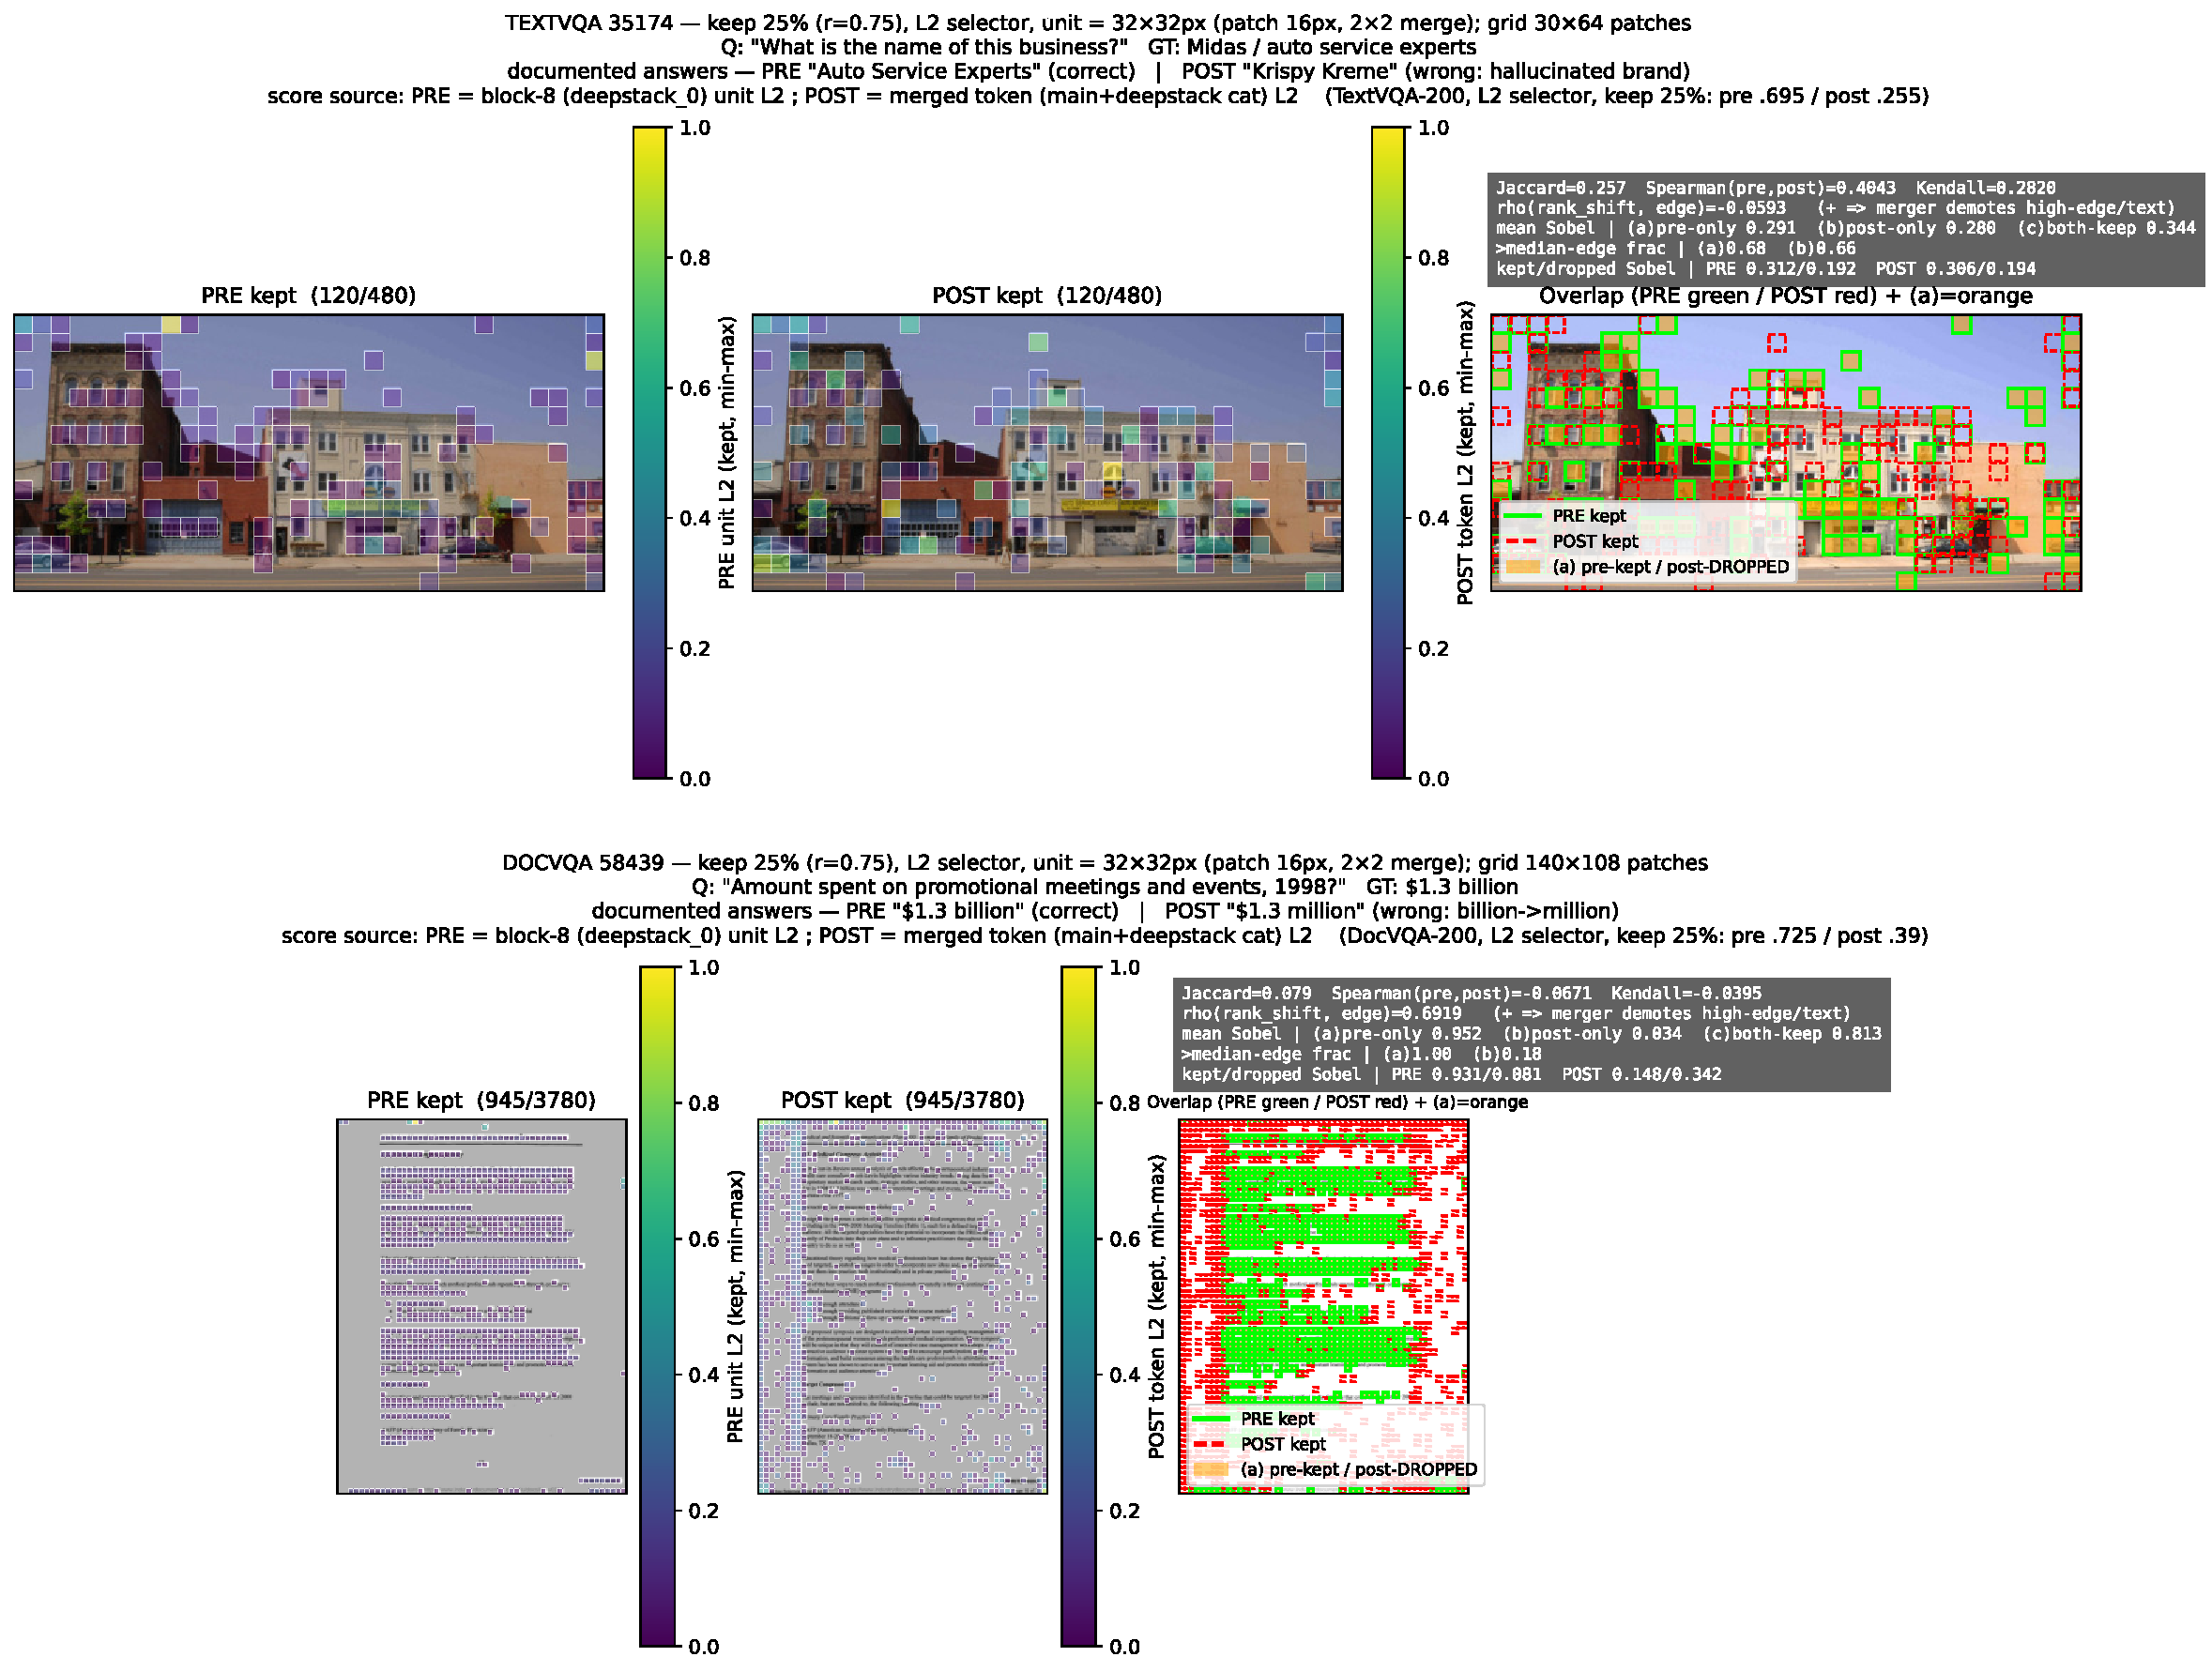
\includegraphics[viewport=387 90 537 283,clip,height=1.65in]{figs/fig4_vector.pdf} &
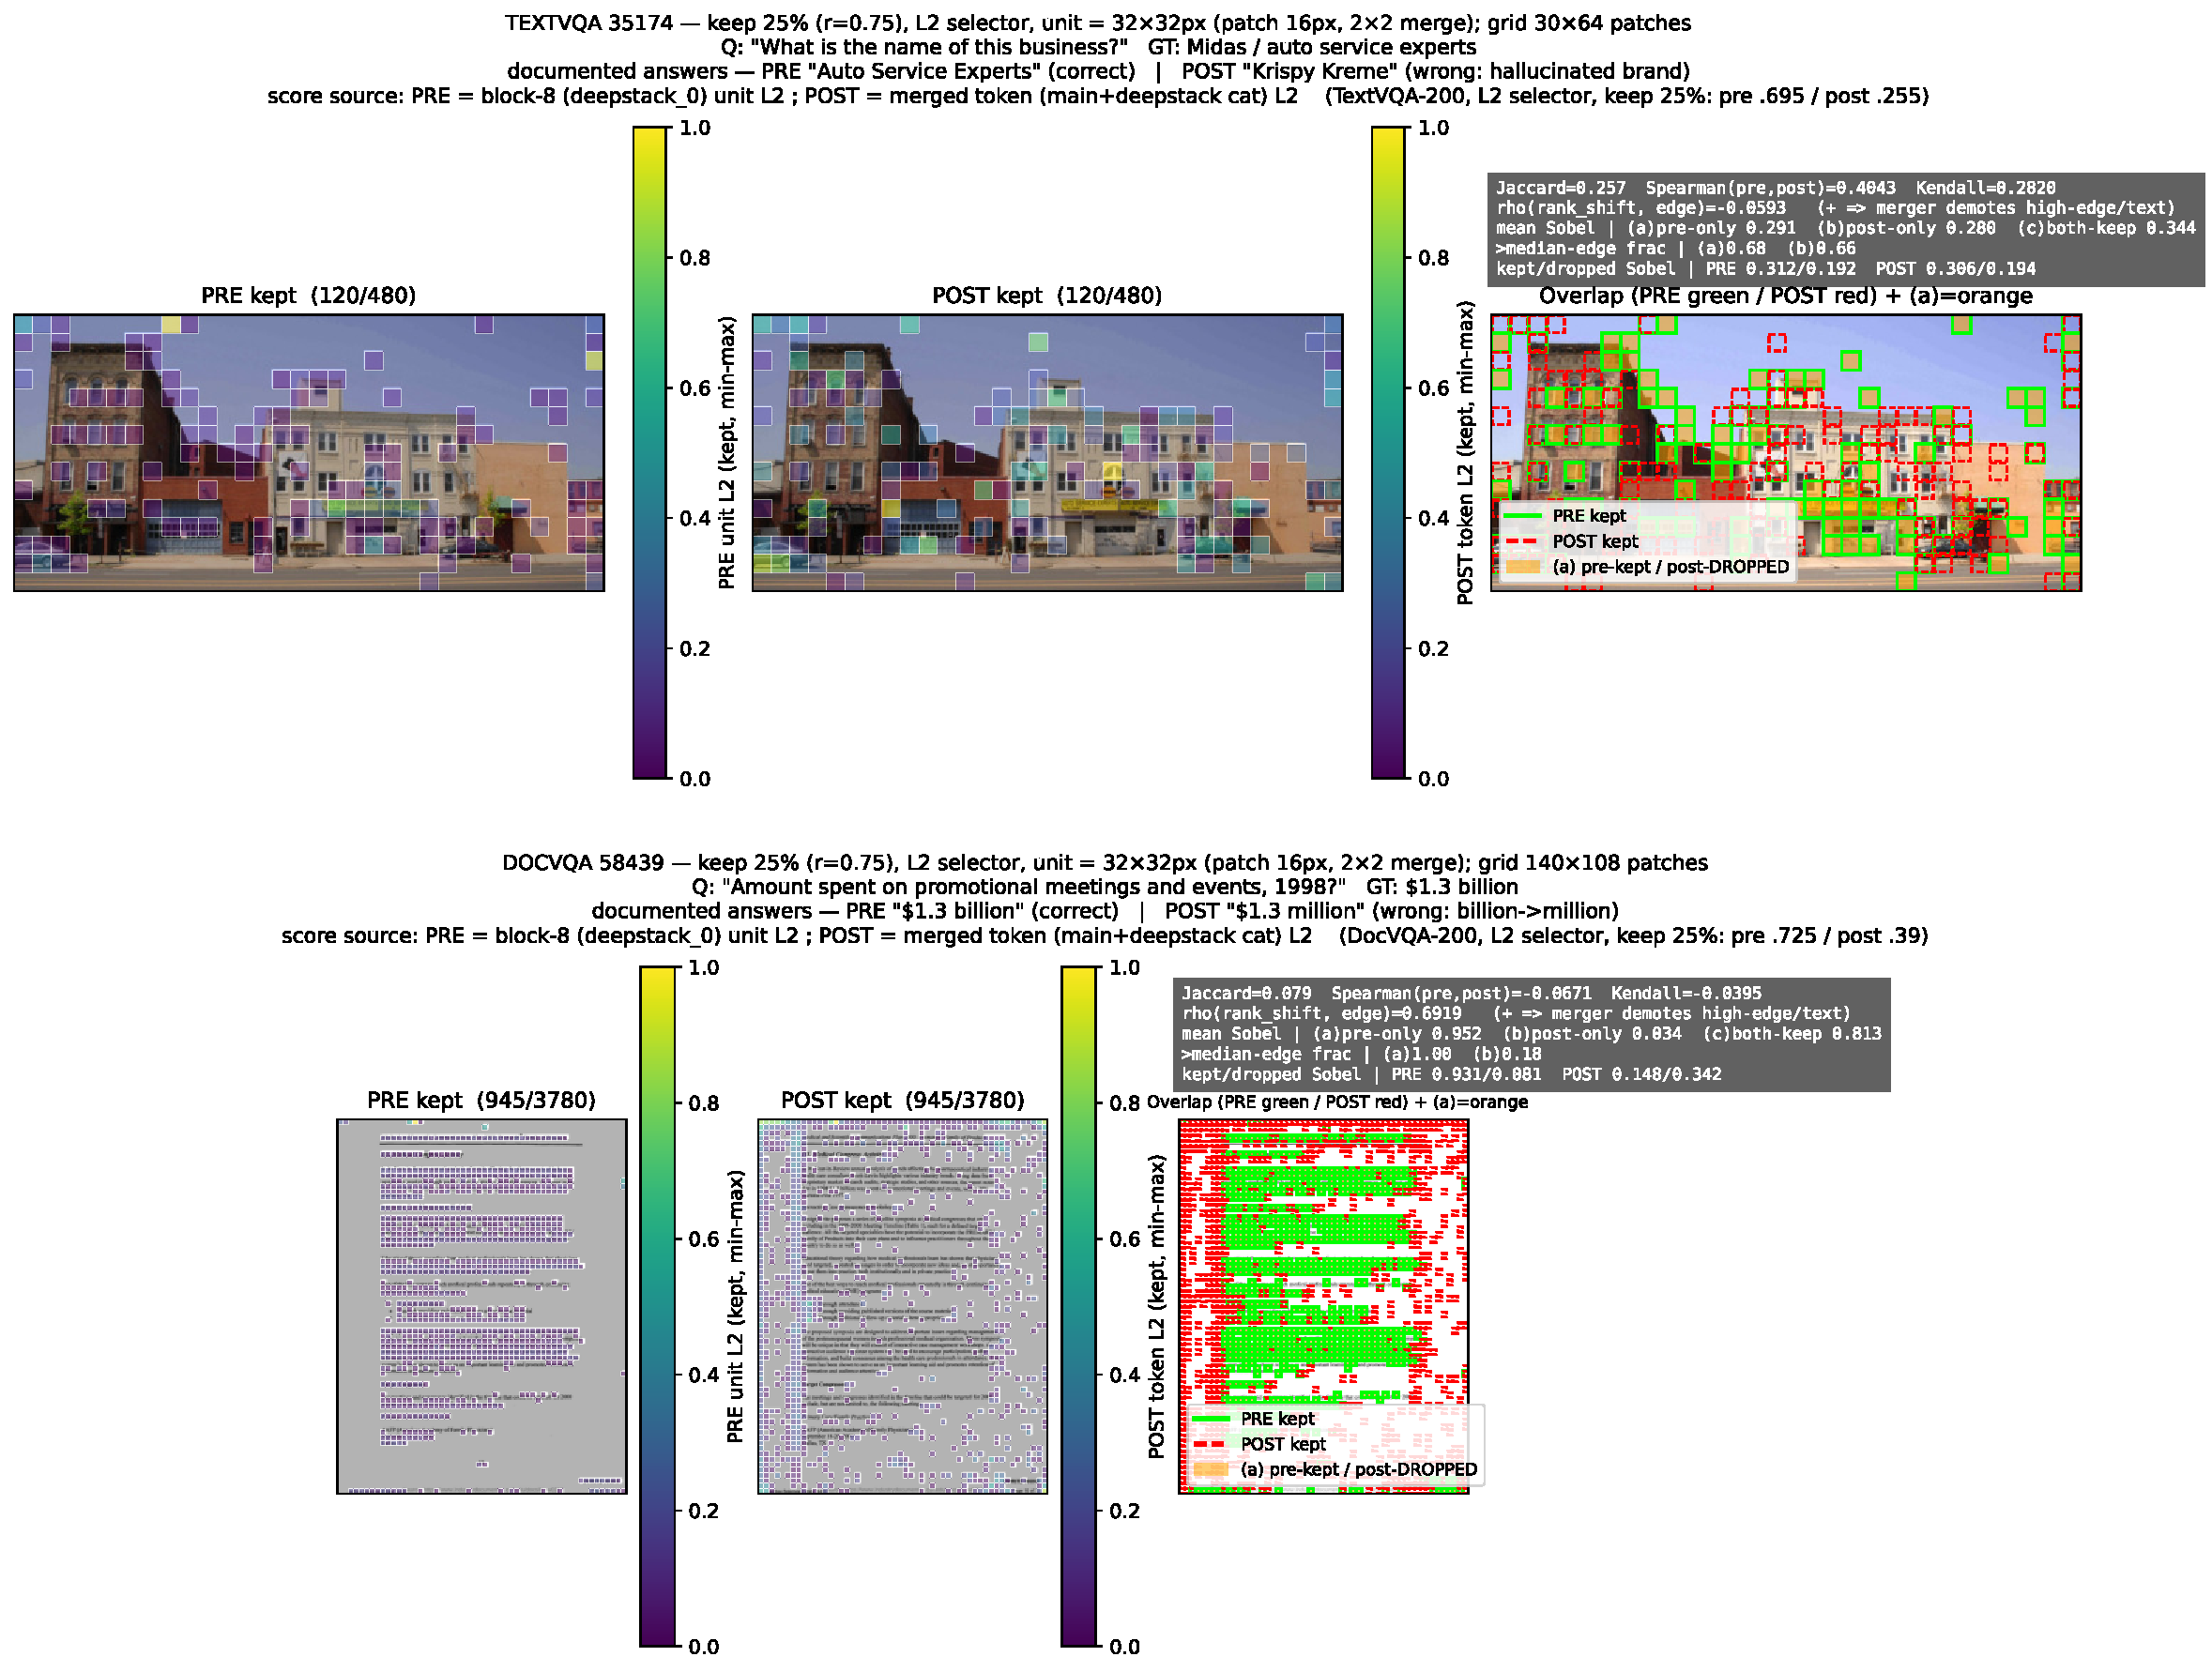
\includegraphics[viewport=603 90 765 283,clip,height=1.65in]{figs/fig4_vector.pdf}
\end{tabular}

\caption{\label{fig:survival}Selected spatial allocations at 25\% retention from the historical $n=200$ TextVQA and DocVQA diagnostics. Columns show early-tap RBM, Post-L2, and their kept-set overlap. Kept-unit colors range from purple to yellow by the norm within each kept set. Overlap marks RBM in green, Post-L2 in red, and RBM-only units in orange.}
\end{figure*}

A ranking-swap check fixes the post-merger computation but substitutes RBM's kept identities. Qwen3-VL kept-set Jaccard overlap is 1.000 on 31 TextVQA and 30 DocVQA probes. Separate 200-example diagnostics show answer agreement on 198/200 TextVQA examples and 200/200 DocVQA examples. These checks show that fixing the retained identities nearly reproduces the deployed outputs. Qwen2.5-VL uses different pre/post ordering conventions; the InternVL3 checks compare accuracy.

\section{Cost and Discussion}
The retained-unit fraction $k/N$ measures the final visual sequence budget. FastV and Hi-Lo process the full visual sequence through early language-model layers; RBM selects before the language model. In the additional HuggingFace implementation, the complete vision transformer and all native merger streams execute before the retained outputs are gathered. Consequently, its input-side ranking does not save vision-encoder or merger computation. Resolution, output length, batching, and backend also determine wall-clock performance.

We measure complete requests on one A40 at batch size one with shared vision SDPA and decoder eager attention. Every path runs in inference mode and projects only the last prefill position to vocabulary logits. A workload fixed before the new results contains 100 TextVQA and 100 OCRBench requests. TextVQA is stratified by the historical retained-count proxy after excluding its five failed inputs; OCRBench uses image-area bands across all 1,000 inputs. Three untimed requests per configuration precede three repetitions of each measured request. Quality is scored on one greedy answer per question, giving two task-specific samples of 100 questions.

Request latency starts from a decoded RGB image before processing and device transfer and ends after the last generated token. It includes full visual encoding, selection or fusion, language-model prefill, and autoregressive decoding. TTFT ends at the first generated token and includes processing and visual computation. CUDA synchronization fixes the measurement boundaries. We take each request's median over its three repetitions before computing workload p50/p95; repetitions are timing replicates. Peak allocated memory is reported in GiB. Whole-workload wall time additionally includes one disk image decode per ID, answer-text decoding, and recording overhead; model loading, warmup, and parity checks are excluded.

Table~\ref{tab:requestcost} reports the complete workload. At 25\% retention, RBM reduces median TTFT from .284 to .164 seconds and median total latency from .421 to .280 seconds. Workload wall time decreases from 428.9 to 329.1 seconds. Peak allocated memory decreases from 22.07 to 17.27 GiB; FastV and Hi-Lo remain near 21.6 GiB, with their early decoder layers processing the full visual sequence. Hi-Lo at 25\% has a .405-second median but a 1.695-second p95 and 427.8-second workload time, compared with 1.652 and 428.9 seconds for None. Median latency, tail latency, and total workload cost therefore give different views of the same compression budget.

All configurations execute the full vision pipeline, whose accumulated wall time is 49.4--49.9 seconds over 600 timed executions per configuration. Hi-Lo's selection adds 25.7 seconds at 25\% retention, measured as CUDA-event elapsed intervals and already included in prefill. Generated output lengths also differ (Table~\ref{tab:requestcost}); decode-time differences contribute to total latency. The separately measured TTFT exposes the cost before autoregressive decoding.

\begin{table*}[t]
\centering
\caption{\label{tab:requestcost}Complete-request costs on the fixed mixed workload of 100 TextVQA and 100 OCRBench requests, repeated three times on one A40. All attempts complete and repeated greedy outputs agree. Total and TTFT show p50/p95 seconds over the 200 per-request medians. Output is the mean generated-token count. Memory is the maximum allocated/reserved GiB over all raw repetitions. Wall time covers all 600 executions plus image decoding and bookkeeping; loading and warmup are excluded.}
\small
\setlength{\tabcolsep}{4pt}
\begin{tabular}{lrrrrrr}
\toprule
Method & Retention & Total (s) & TTFT (s) & Output & Memory (GiB) & Wall (s)\\
\midrule
None & 100\% & .421 / 1.652 & .284 / .734 & 10.31 & 22.07 / 28.06 & 428.9\\
\midrule
\multirow{3}{*}{RBM}
& 25\% & .280 / 1.448 & .164 / .344 & 10.05 & 17.27 / 18.52 & 329.1\\
& 50\% & .317 / 1.473 & .193 / .436 & 10.22 & 18.12 / 20.32 & 356.8\\
& 75\% & .365 / 1.581 & .234 / .557 & 10.28 & 19.81 / 23.53 & 390.0\\
\midrule
\multirow{3}{*}{FastV-k3}
& 25\% & .294 / 1.501 & .174 / .394 & 9.83 & 21.59 / 28.56 & 337.0\\
& 50\% & .335 / 1.520 & .203 / .478 & 10.12 & 21.59 / 28.49 & 364.9\\
& 75\% & .381 / 1.575 & .239 / .587 & 10.38 & 21.58 / 28.13 & 396.9\\
\midrule
\multirow{3}{*}{Hi-Lo}
& 25\% & .405 / 1.695 & .238 / .534 & 10.93 & 21.61 / 28.55 & 427.8\\
& 50\% & .475 / 1.821 & .297 / .699 & 10.77 & 21.61 / 28.56 & 466.7\\
& 75\% & .549 / 1.880 & .372 / .888 & 10.60 & 21.61 / 28.56 & 511.6\\
\bottomrule
\end{tabular}
\vspace{8pt}
\caption{\label{tab:qualitytarget}For each compression method, the measured configuration with lowest p50 among those reaching 95\% of the task subset's None score. Each task has 100 questions. Scores are percentages; OCRBench denotes percent correct on this subset. None is shown as the reference.}
\small
\setlength{\tabcolsep}{5pt}
\begin{tabular}{lrrrrrr}
\toprule
& \multicolumn{3}{c}{TextVQA ($n=100$)} & \multicolumn{3}{c}{OCRBench ($n=100$)}\\
\cmidrule(lr){2-4}\cmidrule(lr){5-7}
Method & Keep & Score (\%) & p50 (s) & Keep & Score (\%) & p50 (s)\\
\midrule
None & 100\% & 81.70 & .396 & 100\% & 78.00 & .713\\
RBM & 50\% & 80.50 & .295 & 50\% & 76.00 & .642\\
FastV-k3 & 25\% & 79.20 & .269 & 75\% & 79.00 & .729\\
Hi-Lo & 75\% & 79.30 & .494 & 75\% & 75.00 & .978\\
\bottomrule
\end{tabular}
\end{table*}

\begin{figure*}[t]
\centering
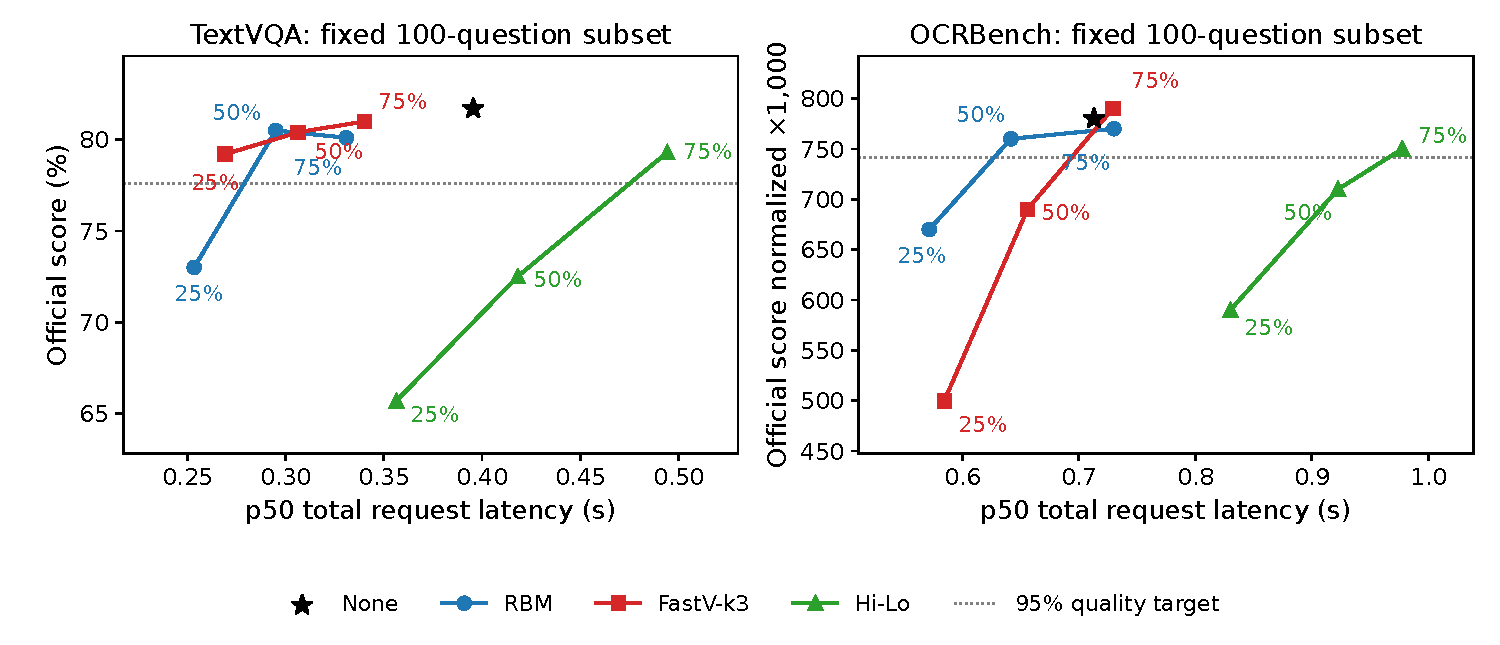
\includegraphics[width=\textwidth]{figs/score_vs_latency.pdf}
\caption{\label{fig:qualitycost}Quality and directly measured request latency on the same fixed 100-question subset of each task, under shared attention. OCRBench values are normalized to 1,000 from these 100 questions. Dotted lines mark 95\% of each subset's None score; labels identify measured retention rates. These are workload-specific point estimates.}
\end{figure*}

Figure~\ref{fig:qualitycost} and Table~\ref{tab:qualitytarget} score the same requests used for timing. Targets are 77.6\% on TextVQA and 74.1\% correct on the OCRBench subset. For each method, we select the measured configuration with lowest p50 among those meeting the target. This gives RBM at 50\%, FastV at 25\%, and Hi-Lo at 75\% for TextVQA; the corresponding OCRBench points are RBM at 50\%, FastV at 75\%, and Hi-Lo at 75\%. Relative to each task's None latency, RBM saves 25.4\% and 10.0\%, respectively. FastV saves 31.9\% on TextVQA but is 2.3\% slower on OCRBench; Hi-Lo is 25.0\% and 37.1\% slower. Meeting the quality threshold consequently does not guarantee lower request cost. The rule compares observed scores on 100 questions per task and does not establish quality equivalence on the full splits.



The main-only control makes stream aggregation central to interpretation. On DocVQA, output scoring can outperform final-input scoring even though the concatenated-output baseline is weaker. The three-model matrix combines the adapter choices in Table~\ref{tab:adapters}; the Qwen3-VL controls expose task-dependent behavior within that architecture. Post-L2 is a diagnostic baseline. In the shared-attention full-split comparison, FastV's TextVQA advantage and RBM's OCRBench advantage likewise give different preferred selectors. RBM exceeds Hi-Lo on TextVQA, while their OCRBench difference remains uncertain. The retention curves quantify substantial recovery as the budget increases, and RBM exceeds both stronger selectors on the DocVQA subset. Hi-Lo's vendored model path remains an implementation difference. The primary full-split and request-cost comparisons fix attention settings; the retention curves and DocVQA stress test retain their attention-backend differences. Direct text-region interventions would additionally test whether a selected unit carries answer-relevant text.

\FloatBarrier
\section{Conclusion}
Native-unit selection reduces language-model visual inputs while reusing a VLM's existing merger and projector interfaces. At 25\% retention, the tested RBM implementations improve text-dense accuracy over their Post-L2 baselines. Qwen3-VL controls show that the preferred scoring representation changes with the task and auxiliary-stream aggregation. Under shared attention, RBM trails FastV on full TextVQA but exceeds it on OCRBench; RBM exceeds Hi-Lo on TextVQA, with an uncertain OCRBench difference. Retention curves and the DocVQA stress test extend these task-dependent comparisons. Complete-request measurements on fixed 100-question task samples show that lower token counts alone do not guarantee lower cost at a target observed quality. Visual token compression should evaluate the scoring representation together with actual token counts, failure coverage, and complete-request cost.

\FloatBarrier
{\small
\bibliographystyle{cvm}
\bibliography{references}
}
\end{document}
